% Request-level KV tiering for capacity-bound decode
% Target: MLSys 2027 (deadline 2026-10-30).
%
% SUBSTRATE: Overleaf is the editor; THIS directory is the source of truth for
% prose (paper/PAPER_PLAN_2026-09-05.md section 8). Figures are built locally
% from paper/data/*.json by paper/figs/*.py and uploaded as PDFs -- they are
% never edited in Overleaf.
%
% CONVENTION, and it is not bureaucracy: every numeric claim carries a
%   % src: <file>.json @ <commit sha>
% comment. Numbers in this project have been measured, retracted and
% re-measured repeatedly; a number without a source is a number we cannot
% defend in a rebuttal.
%
% To build with the real style: drop mlsys2027.sty next to this file
% (from the MLSys 2027 author kit) -- the conditional below picks it up.

\documentclass[letterpaper]{article}

\usepackage{iftex}
% NOTE: do NOT add [accepted] before the camera-ready. In this style family it
% un-anonymises the title block and prints the venue notice; the submission
% build must be anonymous. The title block below is also hand-rolled rather
% than using \mlsystitle/\mlsysauthor, which the real .sty expects -- rework it
% when the author kit arrives, and check the page count then too.
\IfFileExists{mlsys2027.sty}{%
  \usepackage{mlsys2027}%
}{%
  % Local fallback so the draft compiles before the author kit is dropped in.
  \usepackage[margin=1in]{geometry}
  \newcommand{\mlsystitlerunning}[1]{}
  \typeout{WARNING: mlsys2027.sty not found -- compiling in fallback mode.}
}

\usepackage{booktabs}
\usepackage{tikz}
\usetikzlibrary{positioning,arrows.meta,fit,calc}
\usepackage{graphicx}
\usepackage{amsmath}
\usepackage{amssymb}
\usepackage{xcolor}
\usepackage{hyperref}
\usepackage{url}

% Drafting aids. Set \draftfalse before submission; \showtodos triggers an
% error if any TODO survives, so none can ship by accident.
\newif\ifdraft\draftfalse
\ifdraft
  \newcommand{\todo}[1]{\textcolor{red}{[TODO: #1]}}
  \newcommand{\needsgh}[1]{\textcolor{blue}{[GH200: #1]}}
\else
  \newcommand{\todo}[1]{\GenericError{}{UNRESOLVED TODO IN SUBMISSION}{}{}}
  \newcommand{\needsgh}[1]{\GenericError{}{UNRESOLVED GH200 SLOT}{}{}}
\fi

% Shorthands for the analytical spine (section 3). Defined once so the symbols
% cannot drift between sections.
\newcommand{\Xlink}{X}            % interconnect bandwidth
\newcommand{\BW}{\mathrm{BW}}     % achieved HBM bandwidth
\newcommand{\HBM}{\mathrm{HBM}}   % device memory
\newcommand{\Ckv}{C}              % HBM left for KV after weights
% KV bytes per token. Was written $k$ in section 3 and b_tok in sections 1 and
% 6 -- and $k$ is ALSO the rolling-slot depth in the abstract and section 4
% ($k{=}4$, $k/L$), so the same letter carried two meanings a page apart.
% Unified 2026-09-22: b_tok is the bytes, k is the slot depth.
\newcommand{\btok}{b_{\mathrm{tok}}}
\newcommand{\effw}{\eta_w}        % weight-read efficiency
\newcommand{\effkv}{\eta_{kv}}    % paged-KV-read efficiency
% Overlap efficiency: the fraction of a rider's transfer that actually hides
% behind compute. Added 2026-09-22 -- it multiplies the gain law, and every
% earlier estimate of it (0.00, 0.23, 0.38, 0.78, 0.88) came from differencing
% goodput runs that still contained prefill. Only the 4.2b curve measures it.
\newcommand{\effo}{\eta_o}        % overlap efficiency

\begin{document}

% NOTE: do not write \\[1ex] inside \twocolumn[...]. LaTeX scans the optional
% argument to the first unbraced ], so the ] in [1ex] terminates it early and
% the error surfaces as "Argument of \@icentercr has an extra }" -- which
% points at the title, not at the real cause. Use \par\vspace instead.
\twocolumn[
\begin{center}
% Retitled 2026-09-06 for the heterogeneous-memory-system framing. Alternatives
% kept for the co-authors to argue over:
%   "Two Memories, One Pool: Heterogeneous KV Memory for LLM Decode"
%   "Managing HBM and Host DRAM as One KV Memory for LLM Decode"
%   (old, subordinate) "Who Rides Along? Request-Level KV Tiering ..."
{\Large\bf Heterogeneous KV Memory for Capacity-Bound LLM Decode}
\par\vspace{1ex}
% MLSys reviewing is double-blind: the submission carries no author list.
% Replace with the real one for the camera-ready.
{\large Anonymous Author(s)}
\par
{\normalsize Affiliation withheld for review}
\par\vspace{2ex}
\end{center}
]

\begin{abstract}
A decode server's batch is capped by device memory, not arithmetic: KV cache
exhausts HBM long before the arithmetic units are busy, so the GPU runs at
single-digit utilization while turning requests away. Coherent CPU--GPU
interconnects make host DRAM fast enough to hold the KV of an \emph{actively
decoding} request, but existing systems vary how much KV sits on the host and
never \emph{whose} --- they place none, or a uniform fraction of every request.

We present a heterogeneous KV memory that manages HBM and host DRAM as one
store and assigns each request to a tier. A \emph{host-tier} request holds no
device blocks at all: its KV lives in host memory and is streamed in one layer
at a time, just before the attention that consumes it, through a small buffer
that is reused across layers --- so it occupies a few percent of the device
memory a resident request needs. Both tiers are served in a single forward
pass, so the weights are read once however the batch is split, and an admission
controller sizes the host cohort from the link bandwidth and step time it
measures at runtime.

A capacity model then says which configurations this helps. It takes a
profile of the device --- the bandwidth each read achieves, the step time, and
the two costs the host path adds --- and returns the host cohort that maximises
decode throughput. Its content is that the value of a second tier tracks
\textbf{how much of memory the weights consumed}, not model size and not
context length, which cancels.

We implement this in vLLM and measure the costs it turns on: a host-tier
request adds a fixed $12.3$\,ms per step plus $2.2$\,ms per request, so a
prefetch one layer deep hides about $90\%$ of each transfer and a per-step
constant decides the rest. Applied to a Grace-Hopper node the model projects
$\times1.50$ and $\times1.67$ more served requests for the two
weight-heavy configurations, and throughput gains of $\times1.01$ and
$\times1.05$ against margins of a few milliseconds in that constant --- which
is the measurement we ask of such a node, and the one PCIe cannot supply.
\end{abstract}

% ============================================================================
% Section 1 -- introduction.
%
% REFRAMED 2026-09-06 (Ben): the paper is a HETEROGENEOUS MEMORY SYSTEM for
% decode, not "a policy layer on top of somebody's kernel". The old framing was
% structurally subordinate -- it invited "so you wrote the scheduler DirectKV
% skipped" -- and it scattered our pieces as a bag of policies. Under this frame
% the allocator, placement, admission, migration and reclaim are components of
% one system that manages HBM and host DRAM as a single KV memory, and the
% capacity model is that system's design rule.
%
% ALSO CUT 2026-09-06: the losslessness material. Exact placement is what moving
% bytes does; arguing for it invites the doubt it was meant to settle, and no
% comparable systems paper does it.
% ============================================================================

\section{Introduction}
\label{sec:intro}

A GPU serving LLM decode requests is mostly idle. Generating one token for a
batch requires reading every model weight and every resident KV cache byte,
with almost no arithmetic per byte read, so the arithmetic units run at
single-digit utilization while the memory system saturates. What prevents the
server from batching more requests --- which is what would put those units to
work --- is not compute. It is that the KV cache has exhausted device memory. A
recent trace-driven study of production deployments reaches the same conclusion
from the workload side: what binds is ``VRAM capacity, not token
budget''~\cite{bottlenecks}.

The machine, however, has more memory than the GPU's. A Grace-Hopper node pairs
96\,GB of HBM with hundreds of gigabytes of host DRAM, and NVLink-C2C connects
them at 450\,GB/s per direction.\footnote{The commonly quoted 900\,GB/s is
bidirectional; a KV stream is unidirectional host-to-device, so 450\,GB/s is
the figure that bounds it, and we measure rather than assume even that.} At
that rate the KV a decoding request needs can cross the link inside the window
during which the GPU is reading its own weights and wants nothing from the link
at all. Host DRAM stops being a place to park idle requests and becomes usable
memory for running ones.

\paragraph{Two memories, managed as one.} This paper builds a
\textbf{heterogeneous memory system for LLM decode}: HBM and host DRAM managed
as a single KV memory. Its load-bearing decision is \emph{how many} requests to
serve from the host tier, and the answer comes from the interconnect rather
than from memory. A host-tier request must move its entire KV across the link
once per decoded token, so the number that can be sustained is set by what the
link delivers inside a decode step --- a quantity this system measures rather
than declares. Around that decision sit the mechanisms it requires: an
allocator in which a host-tier request holds no device blocks, per-request
placement, and migration between tiers under load.

That framing is not how the field currently treats the second memory. Existing
systems use one memory or the other, statically and totally. Stock vLLM and
SGLang keep 100\% of KV in HBM; when it does not fit, requests wait. DirectKV,
which contributes the zero-copy attention kernel that makes host-resident KV
efficient at all, keeps 100\% on the host for every request always --- its \S6
stores each layer's initial $K,V$ in CPU memory during prefill and its Alg.~3
appends new $K,V$ there during decode. That is precisely why it needs no
memory management: placement is static and total, and its \S8.1 says the design
``does not change scheduling, batching, or KV-management policies.''

Neither is optimal, for a reason visible without measurement. An all-HBM server
reads KV at HBM bandwidth and leaves the interconnect idle. An all-host server
reads KV over the interconnect and leaves the HBM not holding weights idle. A
system that places some requests in each reads from both at once, and its batch
is bounded by the sum:

\begin{table}[t]
\centering
\small
\begin{tabular}{lrr}
\toprule
\emph{Projected.} Qwen2.5-32B fp16, 8K, GH200-96 & KV read per step & batch \\
\midrule
all-HBM (vLLM, SGLang)      & 26.5\,GB HBM, \textbf{0 link} & 12 \\
all-host (uniform offload)  & \textbf{0 HBM}, 8.8\,GB link & 4 \\
\textbf{both (this paper)}  & 26.5\,GB HBM \textbf{+} 8.8\,GB link & \textbf{16} \\
\bottomrule
\end{tabular}
\caption{Each single-memory design leaves one of the two KV paths unused.
Weight traffic is identical in all three rows and excluded, so the column
compares like with like. \textbf{These are projections}, computed by
\texttt{model/killer\_v2.py} from: measured checkpoint $W = 65.5$\,GB, a 4\,GB
device reserve for activations and fragmentation, hence $\Ckv = 26.5$\,GB;
$\btok = 256$\,KiB so a request at 8K holds 2.15\,GB; $\mathrm{ITL}_0 = 33.9$\,ms
from Eq.~\ref{eq:step}; $\Xlink = 419$\,GB/s, the measured host-to-device rate
on this part~\cite{pie}, not the 450\,GB/s spec figure; and $\effo = 0.62$.
The last is the weakest input: it is measured on A100/PCIe
(\S\ref{sec:eval:cost}) and assumed to carry to a coherent link, which is the
first thing \S\ref{sec:eval} asks of one. At $\effo = 1$ the host row would
read 6 and the total 18.}
\label{tab:endpoints}
\end{table}

Writing that sum out states the contribution exactly. For requests of $S$
tokens at $\btok{}$ KV bytes each, the resident cohort is a
\emph{memory} quantity and the host cohort is a \emph{bandwidth} one:
%
\begin{equation}
B \;=\; \underbrace{\frac{\Ckv}{S\,\btok{}}}_{\text{device capacity}}
\;+\;
\underbrace{\frac{\mathrm{ITL}\cdot\Xlink\cdot\effo}{S\,\btok{}}}_{\text{interconnect}}
\label{eq:two-terms}
\end{equation}
%
The second term does not contain $\Ckv$. Admission is thereby decoupled from
device capacity and bounded instead by what the link can deliver within a step
--- which is the decision this paper is about, and the one no existing system
makes: the endpoints in Table~\ref{tab:endpoints} set the host cohort to zero
or to everything, neither of which consults the interconnect at all.

\paragraph{When is a second memory tier worth having?} Before building one we
ask when it pays, and the answer is sharply bounded. We derive a closed-form
capacity multiplier $1 + (\Xlink/\BW)\,\effo\,(\HBM/\Ckv)$, where $\Ckv$ is the
device memory left after weights and $\effo$ is the fraction of a rider's
transfer that overlaps compute, and validate its structure against 54 measured
configurations. Two consequences contradict the obvious intuition. Long context
does \emph{not} help: it shrinks the HBM-resident cohort and the affordable
host cohort in the same proportion, leaving their ratio unchanged. And the
value of a second tier tracks \textbf{how much of memory the weights ate},
not model size. An 8B model leaves so much HBM free that there is nothing to
buy; a 32B model at fp16 leaves 28\,GB and gains materially. The sharpest
demonstration is that \emph{the same model at two weight precisions} lands at
two different points on the curve.

The model earns its place by explaining a published result its own authors do
not. DirectKV reports being ``slightly slower than SGLang'' on Llama-3.1-8B and
winning on OPT-13B/30B ``where SGLang OOMs''. Our capacity multiplier predicts
that inversion from the two models' weight footprints alone. A design rule that
accounts for when the technique \emph{fails} is worth more than one tuned to
its successes.

\paragraph{Contributions.}
\begin{enumerate}
\item \textbf{A capacity model for heterogeneous KV memory}
      (\S\ref{sec:model}): a closed-form multiplier and an applicability gate,
      validated on hardware and against a published system's own results. Both
      exclude configurations the field currently evaluates on.
\item \textbf{A two-tier KV memory manager} (\S\ref{sec:design}) in which a
      host-tier request holds no device blocks at all, so tiered requests are
      additive rather than substitutional --- the property that makes the
      interior point of Table~\ref{tab:endpoints} reachable.
\item \textbf{Admission decoupled from device capacity and bounded by the
      interconnect} (\S\ref{sec:design}): the host cohort of
      Eq.~\ref{eq:two-terms} sized from a per-step transfer budget that is
      \emph{measured} --- from the rider-free step time and the achieved link
      bandwidth --- rather than declared as a constant. We show by ablation
      that this derived count, and not a fixed offload fraction, is what
      carries the result.
\item \textbf{An implementation in vLLM v1 and an evaluation separating the
      memory system's contribution from the kernel's} (\S\ref{sec:eval}), by
      running uniform offload and our manager on one substrate, together with
      two negative results we report rather than bury: per-request placement
      driven by observable state did not separate from arrival order on our
      substrate --- and context length, the intuitive signal, does not
      discriminate at all --- while closed-loop migration measured its own
      demotions as harmful and reverted them.
\end{enumerate}

We state the last of these deliberately. A host tier admits a policy design
space --- which requests to move, and when to move them --- and we built that
space and report that, at the rider counts a PCIe-class link permits, it does
not yet pay. A policy choosing among two candidates cannot demonstrate value;
whether it does so when the budget admits dozens is a question for a coherent
interconnect, not a claim we make here.

\paragraph{Scope.} We target a decode node in a prefill/decode-disaggregated
deployment~\cite{distserve,splitwise,mooncake}, where a request arrives with
its KV already computed. \S\ref{sec:background:pd} explains why that assumption
is what makes host-tier requests additive.

\paragraph{Results.} On A100/PCIe --- the regime our own model says cannot pay
--- the memory system works and the economics do not. Against a fixed KV pool,
host-tier requests raise peak concurrency from 8 to 48, itself a lower bound
since 48 was the entire offered load.
% src: paper/data/preload_capacity.json @ f3df05bdb
In a separate experiment that isolates a rider's cost --- riders added on top of
a fixed resident batch, with prefill cancelled by construction --- only
$\effo = 0.62$ of a host-tier request's transfer overlaps compute, and the
unhidden residual costs $8.3$\,ms of a $54$\,ms step, leaving decode throughput
$0.86\times$ that of not offloading at all.
% src: paper/data/rider_cost_4p2b.json @ 21ea9b18d
End to end, through the prefill handover, the deficit is $2.3\%$.
% src: paper/data/pd_decode_goodput.json @ f3df05bdb
That is what the model predicts for a 25\,GB/s link, and DirectKV reaches the
same boundary from the kernel side, concluding that on PCIe theirs ``should be
viewed primarily as a capacity-extension mechanism''. It fixes one end of the
bandwidth axis.
On a coherent interconnect we report the same comparison at matched latency
targets, together with the second point on the bandwidth axis that turns the
cost decomposition of \S\ref{sec:eval:cost} into a law with a measured
crossing rather than an extrapolated one.

% ============================================================================
% Section 2 -- background and system model.
%
% STATUS: first full draft, 2026-09-05.
%
% This section carries the paper's largest reviewer risk (plan section 6.1).
% Riders are admitted with ZERO main-pool blocks and their prompt declared
% already computed. That is only legitimate on a decode node whose KV arrives
% from a prefill node. Stated here it is a scoping assumption about the
% architecture the field already runs; discovered by a reviewer in the
% evaluation it reads as concealment.
% ============================================================================

\section{Background and system model}
\label{sec:background}

\subsection{Capacity, not compute, caps the batch}

A decode step is memory-bound by a wide margin. It reads every model weight
once and every resident KV byte once, and performs arithmetic whose intensity
equals the GQA group size --- 4 to 8 on current models, against a balance point
of order $100$ FLOP/byte on the accelerators in question (116 on an H100, 98 on
the A100-80 we measure). The consequence is that a decode engine runs at
single-digit arithmetic utilization, and what stops it running a larger batch
is not the arithmetic but the bytes: KV cache exhausts the device long before
the streaming multiprocessors (SMs) saturate. A recent trace-driven study of production serving reaches the
same conclusion from the workload side, finding that ``VRAM capacity, not token
budget'' is what binds~\cite{bottlenecks}.

Which of the two reads dominates that step is a property of the model, not of
the operating point, and the spread is large. At a full pool on an A100-80,
Llama-3.1-8B spends $10.5$ of $79.3$\,ms reading weights --- 13\% weights,
87\% KV --- while Qwen2.5-32B spends $42.9$ of $55.7$\,ms, which is 77\%
weights and 23\% KV.
% src: paper/model/p4_llama8b_a100.json, p4_qwen32b_a100.json @ 2bfc6ca5e
Both are capacity-bound, and they sit at opposite ends of the same axis on
identical hardware.

That spread is what makes a second tier worth having, and the direction is the
opposite of the intuitive one. The weight read is a \emph{fixed} per-step window
during which the link carries nothing: the GPU is streaming parameters and wants
no KV. The larger the weights are relative to the device, the longer that window
is, and the less HBM is left for resident KV --- so the very configurations where
weights dominate the step are the ones with both the most idle link time to
exploit and the least device memory to exploit it with. Qwen2.5-32B is the
favourable case here \emph{because} it is 77\% weights, and Llama-3.1-8B is
unfavourable because it is 13\%. \S\ref{sec:model} makes that statement
quantitative, and \S\ref{sec:model:omits} gives the cost that can cancel it.

\subsection{Host memory as a tier for actively decoding requests}

Offloading KV to host memory is an old idea that a new interconnect has
changed. Over PCIe~4 at roughly 25\,GB/s, streaming a request's KV to the GPU
every decode step costs more than the step itself, so host memory could only
ever be a \emph{swap} target: somewhere to park a request that is not currently
running. NVLink-C2C moves 450\,GB/s in each direction,\footnote{The commonly
quoted 900\,GB/s is bidirectional. A KV stream is unidirectional
host-to-device, so 450\,GB/s is the figure that bounds it, and we measure
rather than assume even that.} and at that rate the bytes a decoding request
needs can cross the link inside the time the GPU spends reading its own
weights.

That changes what host memory \emph{is}. It becomes a tier that an
\emph{actively decoding} request can occupy, which is a state that did not
previously exist and which no existing KV policy governs --- continuous
batching, prefix reuse, eviction and hierarchical caching all decide the
residency of blocks belonging to requests that are not currently running.

It also changes what the movement should be. \emph{Swapping} relocates
ownership: a unit of KV lives on one side, is brought over to be used, and must
be written back if it changed --- so every offloaded byte crosses the link twice
per generated token, once in each direction. \emph{Streaming} keeps the host
copy authoritative and treats the device-side copy as a cache, so the return
leg carries only the token just produced. The distinction costs a factor of two
in interconnect pressure on the resource that bounds the whole technique, and
it follows from what the offloaded unit \emph{is} rather than from any
optimisation; \S\ref{sec:related} works it through against the systems that
made each choice.

\subsection{System model: a disaggregated decode node}
\label{sec:background:pd}

We target a \textbf{decode node in a prefill/decode-disaggregated
deployment}~\cite{distserve,splitwise,mooncake}. Prefill runs on separate
hardware; a request arrives at the decode node with its KV cache already
computed, delivered over the cluster transport. This is the production default
rather than a convenience we adopt: the separation exists because prefill and
decode have opposite resource profiles, and every major serving stack now
supports it.

The assumption does real work here, and we state exactly what it buys. On a
decode node, a host-tier request's KV can be delivered \emph{into host memory}
and never occupy an HBM block at all --- not even transiently. Riders are
therefore \textbf{additive}: they are served in addition to a full resident
cohort rather than displacing part of it.

In a combined prefill+decode engine this is false, and the difference is not
subtle. A request must be prefilled somewhere, so its KV lands in HBM first and
is only reclaimed afterwards; riders and residents then draw on the same
headroom, and we measured the result --- the served total creeps toward the
all-HBM capacity from below and never passes it, at any setting of the
resident-cohort cap. A rider whose prefill stays resident frees nothing while
still costing interconnect bandwidth every step, which is strictly worse than
leaving it in HBM. We report that negative result in
\S\ref{sec:eval:capacity}, because it is what motivates the mechanism and
because it bounds where the technique applies.

The assumption's cost is that KV must reach host DDR. We do not wave this
away: \S\ref{sec:impl:stash} implements the handover and \S\ref{sec:eval}
reports what it costs, so the reader can price the assumption rather than
accept it.

% NOTE: a subsection defining "lossless" and describing how we verify it was
% removed 2026-09-06. Exact placement is a property of moving bytes rather than
% approximating them, and no comparable systems paper argues for it -- doing so
% invites the doubt it was meant to settle. The bf16 near-tie methodology, which
% is a real gotcha, now lives as one paragraph in the evaluation setup where it
% belongs.

% ============================================================================
% Section 3 -- the analytical spine. Contribution 1.
%
% STATUS: first full draft, 2026-09-05. This section survives every branch of
% the GH200 gate (paper/PAPER_PLAN_2026-09-05.md section 4) and is deliberately
% written first. Claims C2, C3, C4.
%
% All numbers here: % src: paper/model/p4_*.json @ 2bfc6ca5e
% ============================================================================

\section{When does host-KV offload pay?}
\label{sec:model}

Before describing a policy we establish what there is to gain, because the
answer is narrow and the boundaries are sharp. This section derives four
closed-form results, reports which of them survived contact with hardware, and
uses the survivors to explain a published result that its own authors leave
unexplained.

\subsection{Setup}

Let $\Xlink$ be the achieved interconnect bandwidth between host memory and the
GPU, $\BW$ the achieved HBM bandwidth, $\HBM$ the device memory, $W$ the bytes
of model weights, and $\Ckv = \HBM - W - \mathcal{R}$ the memory left for KV cache, where
$\mathcal{R}$ is a device reserve for activations, workspace and allocator
fragmentation ($4$\,GB on the parts we consider). Every equation and table below
uses this definition. Let $S$
be the context length and $\btok{}$ the KV bytes per token.

A decode step reads every weight once and every resident KV byte once. Writing
$\effw$ and $\effkv$ for the fraction of peak bandwidth each achieves --- we
show below that these differ, and that the second is not a constant --- the
step time at batch $B$ is
%
\begin{equation}
\label{eq:step}
\mathrm{ITL}(B) \;=\; \frac{W}{\BW \cdot \effw} \;+\; \frac{B \cdot S \cdot \btok{}}{\BW \cdot \effkv}.
\end{equation}
%
The capacity-limited batch is $B_{\mathrm{cap}} = \Ckv / (S \btok{})$: the point at
which KV, not arithmetic, exhausts the device. A rider's KV lives in host memory
and streams over the interconnect during the step. A step of length
$\mathrm{ITL}$ cannot carry more than $\mathrm{ITL}\cdot\Xlink$ bytes across the
link whatever else is true, so the rider cohort is bounded by
%
\begin{equation}
\label{eq:boff}
B_{\mathrm{off}} \;=\; \frac{\mathrm{ITL} \cdot \Xlink}{S \btok{}}.
\end{equation}
%
This is a \emph{capacity} bound and nothing more: it says how many riders' bytes
fit, not what they cost. The transfer is issued one layer ahead of the attention
that consumes it, and the fraction of its time that does \emph{not} reappear as
added step time is the \textbf{overlap efficiency} $\effo \in (0,1]$. Perfect
overlap is the exception --- on A100/PCIe we measure $\effo = 0.62$
(\S\ref{sec:eval:cost}) --- but $\effo$ does not belong in this equation. It
describes what the bytes cost once carried, not how many fit, and charging it
here as well as in the throughput form (\S\ref{sec:model:omits}) would count it
twice.

\subsection{(a) Context length cancels}
\label{sec:model:cancel}

The ratio of riders to residents,
%
\begin{equation}
\label{eq:cancel}
\frac{B_{\mathrm{off}}}{B_{\mathrm{cap}}}
  \;=\; \frac{\mathrm{ITL}\cdot \Xlink / (S \btok{})}{\Ckv / (S \btok{})}
  \;=\; \frac{\mathrm{ITL}\cdot \Xlink}{\Ckv},
\end{equation}
%
is independent of $S$. Long context does not make offloading more attractive:
it shrinks both cohorts equally. This is worth stating because the intuition
runs the other way --- long context is what makes KV cache expensive, so it
seems like the regime where moving KV off-device should pay most. It is not.
What a long context buys the rider in freed HBM, it spends again in per-step
transfer.

\paragraph{Validated on hardware, per model.} Equation~\ref{eq:step} makes two
claims: that ITL depends on batch and context only through their product
$B\cdot S$, and that the intercept is the weight term $W/(\BW\effw)$. We test
them on an A100-80 over 41 single-shot configurations --- 27 on Llama-3.1-8B, 14
on Qwen2.5-32B --- plus 13 three-repeat points drawn from the same grid.

Within each model, ITL is linear in $B\cdot S$: $R^2 = 0.975$ for Llama-3.1-8B
with residuals unbiased across $S \in \{2048, 4096, 8192\}$ (means $+0.09$,
$-0.09$, $+0.00$\,ms), and $R^2 = 0.92$ for Qwen2.5-32B. $B{=}16,S{=}4096$ and
$B{=}8,S{=}8192$ both measure $17.17$\,ms. \textbf{Pooling the two models is
meaningless and we do not report it} --- the fit across both is $R^2 = 0.19$,
because Eq.~\ref{eq:step}'s intercept is model-dependent, which is the whole
content of \S\ref{sec:model:modeldep}.

That intercept is the sharper test, because Eq.~\ref{eq:step} predicts it rather
than fitting it. The fitted intercepts are $9.4$\,ms for Llama-3.1-8B and
$43.6$\,ms for Qwen2.5-32B; $W/(\BW\effw)$ at the measured peak of
$1935$\,GB/s and $\effw = 0.75$ predicts $11.1$ and $45.2$\,ms. Agreement is
within $1.7$\,ms across a $4\times$ range of weight footprint, and the two
errors have \emph{opposite} signs, which is what a shared miscalibration would
not produce.

The residual is mostly one thing, and it is worth reporting because it
contradicts a simplification we make elsewhere. \textbf{$\effw$ is not a single
constant}: the $B{=}1$ points give $0.712$ for Llama-3.1-8B and $0.773$ for
Qwen2.5-32B, an 8.6\% spread. Using each model's own value the predictions move
to $11.7$ and $43.8$\,ms, which improves Qwen to $0.2$\,ms and worsens Llama to
$2.3$. So the single-$\effw$ approximation is the better predictor of the two,
and we keep it while recording that it is an approximation across models rather
than a measured constant --- Appendix~\ref{app:params} gives the per-model
figures.
% src: paper/model/p4_llama8b_a100.json, p4_qwen32b_a100.json @ 2bfc6ca5e
We use differential timing --- $\mathrm{ITL} = [T(N_2) - T(N_1)]/(N_2 - N_1)$
with identical prompts in both runs, so prefill and warmup cancel; context
grows across the $N_2-N_1$ tokens, which the differencing does not remove.

\subsection{(b) The step time is model-dependent}
\label{sec:model:modeldep}

At capacity a step reads all of device memory once, which invites the
simplification $\mathrm{ITL}_0 \approx \HBM/\BW$: a quantity fixed by the
device alone. It does not hold. Evaluating Eq.~\ref{eq:step} at each model's
own pool gives a full-pool ITL of $79$\,ms for Llama-3.1-8B against $56$\,ms for
Qwen2.5-32B --- a $1.4\times$ spread across two models on identical hardware.
These two are \emph{projections}, not measurements: the largest working sets we
could fit on an 80\,GB part measure $69.7$ and $50.9$\,ms, and the full-pool
points extrapolate the $\effkv$ curve of \S\ref{sec:model:params} beyond them.
% src: paper/model/p4_llama8b_a100.json @ 2bfc6ca5e
% src: paper/model/p4_qwen32b_a100.json @ 2bfc6ca5e
% NOTE: the full-pool step times are EXTRAPOLATED from these files via the
% eff_kv curve of appendix A, not read from them. Largest measured: 69.7 and
% 50.9 ms. The cause is that
weights and paged KV do not stream at the same efficiency
(\S\ref{sec:model:params}): a model that is mostly weights reads device memory
faster than one that is mostly KV, so $\mathrm{ITL}_0$ depends on the
weight-to-KV ratio and the applicability gate in (d) is model-dependent rather
than a property of the device.

The transfer budget is still $\mathrm{ITL}\cdot\Xlink$, and most of it is still
bought with \emph{weight-read time}. On GH200, Qwen-32B spends roughly
21\,ms of a 34\,ms step reading weights, during which nothing else contends for
the interconnect. The opportunity is time, not spare bandwidth. It is not free,
though: the arriving bytes are written into HBM, and those writes consume device
bandwidth during a step that is already HBM-bound.

\subsection{(c) The gain law}
\label{sec:model:gain}

Adding $B_{\mathrm{off}}$ riders to $B_{\mathrm{cap}}$ residents multiplies the
served batch by
%
\begin{equation}
\label{eq:gain-exact}
\text{gain} \;=\; 1 + \frac{B_{\mathrm{off}}}{B_{\mathrm{cap}}}
      \;=\; 1 + \frac{\mathrm{ITL}_0 \cdot \Xlink}{\Ckv}.
\end{equation}
%
That is exact in the fluid limit, and it is the form to compute with. To read the
\emph{structure} off it, substitute the full-pool step time
$\mathrm{ITL}_0 \approx \HBM/(\BW\,\bar\eta)$, where $\BW$ is now the device's
\textbf{peak} bandwidth and $\bar\eta$ the pool-weighted read efficiency it
actually achieves (\S\ref{sec:model:params}):
%
\begin{equation}
\label{eq:gain}
\text{gain} \;\approx\; 1 + \frac{\Xlink}{\BW\,\bar\eta}
                          \cdot\frac{\HBM}{\Ckv}.
\end{equation}
%
$\bar\eta$ must be carried. Dropping it --- which is easy to do, since it
cancels visually against $\BW$ --- understates the gain by about 10\% across
Table~\ref{tab:gain} (9.9\% to 11.4\%), because $\bar\eta$ runs 0.52--0.73
rather than 1. The
bandwidth ratio $\Xlink/\BW$ is a handicap --- $419/4000 = 0.105$ against peak
even on NVLink-C2C --- and it cannot be improved by anything a serving system
does. The amplifier is
$\HBM/\Ckv$: \textbf{the value of offloading tracks how much of HBM the weights
ate}, not model size and not context length.

That single observation is the section's most useful consequence, because it
is counter to how the field selects evaluation models.

Equation~\ref{eq:gain} is a \emph{capacity} result: it counts requests the
device can hold, not requests per second it can serve. Two effects separate the
two, and \S\ref{sec:model:omits} charges both. Each rider costs $k/L$ of a
resident's blocks for the rolling window it streams into, so the resident cohort
shrinks slightly as the host cohort grows --- which is why
Table~\ref{tab:gain}'s capacity column ($\times$1.48 for Qwen2.5-32B fp16) sits
below a hand recomputation of Eq.~\ref{eq:gain} ($\times$1.54). And the unhidden
fraction $(1-\effo)$ of every rider's transfer lands on the step. Neither is
negligible, and the second is what decides the paper.

\begin{table*}[t]
\centering
\small
\begin{tabular}{lrrrrrr}
\toprule
Model (GH200-96) & weights & $\Ckv$ & $\HBM/\Ckv$ & ITL$_0$ & capacity & tput \\
\midrule
Llama-8B fp16          & 16.1\,GB & 75.9\,GB & 1.26 & 46.6\,ms & $\times$1.03 & $\times$0.78 \\
Qwen-32B \textbf{fp8}  & 32.0\,GB & 60.0\,GB & 1.60 & 43.3\,ms & $\times$1.09 & $\times$0.78 \\
Qwen-32B \textbf{fp16} & 65.5\,GB & 26.5\,GB & 3.63 & 33.9\,ms & $\times$1.45 & $\times$0.85 \\
Llama-70B fp8          & 72.7\,GB & 19.3\,GB & 4.97 & 33.0\,ms & $\times$1.73 & $\times$0.97 \\
\bottomrule
\end{tabular}
\caption{\emph{All rows are projections}, not measurements. A second memory
tier is an amplifier on $\HBM/\Ckv$ and the table is monotone in it.
$\Ckv = \HBM - W - 4$\,GB, the last term a device reserve for activations,
workspace and allocator fragmentation --- so weights and $\Ckv$ do not sum to
$\HBM$, and Eq.~\ref{eq:gate} uses the same definition. \emph{capacity} is
$B_{\mathrm{tot}}/B_0$, charging both the $k/L$ of a resident's blocks each
rider displaces at $k{=}4$ \emph{and} the two HBM passes its KV makes per step
(the link writes it into the slot, attention reads it out). \emph{tput} is
Eq.~\ref{eq:gain-tput}, which additionally charges $F = 12.3$\,ms and the
unhidden residual $\Delta$ (2--13\,ms across these rows). \textbf{Every row
loses on tput while every row gains on capacity}: that gap, not the multiplier,
is the paper's result, and \S\ref{sec:model:omits} says what would close it.
Charging the HBM passes is what separates the two small-amplifier rows from the
two large ones --- uncharged they read $\times$1.22 and $\times$1.28 --- so the
amplifier matters \emph{more} once a rider is billed for the device bandwidth
it actually consumes, not less. Weight figures are
measured checkpoints except Qwen-32B fp8, for which we hold no checkpoint and
quote the nominal size; the fp16 row measures 65.5\,GB against a nominal 64.0,
so the fp8 row is likely optimistic by a similar margin. \textbf{The two
Qwen-32B rows differ only in weight precision}, which isolates $\HBM/\Ckv$ from
every other architectural variable.}
% src: paper/model/tables.py @ this commit (wraps model/killer_v2.py:analyze,
% S=8192, GH200-96 at the measured 419 GB/s, slo=50 ms, stage=0, eta_o=0.62)
\label{tab:gain}
\end{table*}

\paragraph{Weight precision is the clean lever on $\HBM/\Ckv$, and we do not
pull it.} Comparing models of different sizes moves the weight footprint, but
also layer count, KV-head count and architecture, so a trend across 8B, 32B and
70B confounds the quantity the law is about with three others. The clean
instrument is a \emph{single} model at two weight precisions, which moves
$\HBM/\Ckv$ and nothing else --- the two Qwen-32B rows above share an
architecture, a tokenizer and a KV geometry and differ only in that fp8 weights
leave 60.0\,GB for KV where fp16 leave 26.5\,GB.

We report those rows as projections rather than measurements. Validating the
$\HBM/\Ckv$ axis directly would have cost hours we judged better spent
comparing against the closest prior system, so the law is validated across
\emph{bandwidth} (\S\ref{sec:eval:cost}) while its amplifier rests on the
parameter fit and on agreement with published results
(\S\ref{sec:model:directkv}). \S\ref{sec:eval:model} states this again where
a reviewer will look for it.

The same observation has a practical edge, which \S\ref{sec:discussion} takes
up: quantizing \emph{weights} is not neutral to a memory system, it actively
removes its headroom, while quantizing \emph{KV} scales both cohorts together
and composes.

\paragraph{What is and is not held out.} $\effw$ is calibrated on the $B{=}1$
points, where the KV term is negligible, and $\effkv$ on sub-capacity working
sets, so the two come from disjoint parts of the same sweeps. The full-pool step
times above are \emph{not} an independent check on them --- they are computed
from those same fits, so comparing Eq.~\ref{eq:step} against them would be
circular and we do not. The genuine out-of-sample test is the intercept
recovery of \S\ref{sec:model:cancel}: $\effw$ fitted at $B{=}1$ predicts the
intercept of a regression over the whole grid, on both models, to within
$1.1$\,ms. Measuring a real full-pool step on a device large enough to hold one
would be the stronger test, and we have not run it.

Several of these parameters are measured with error, so it is worth asking
which ones the projection actually depends on. For Qwen-32B fp16 on GH200-96 at
8K --- where Table~\ref{tab:gain} reads $\times1.45$ --- $\effw$ over 0.70--0.80
barely moves it, spanning $\times1.41$--$\times1.50$. \textbf{$\effkv$ is a
different matter}: $\pm20\%$ spans $\times1.31$--$\times1.64$. Charging the
rider's HBM passes is what made it so, because $\effkv$ now prices the rider
traffic as well as the resident cohort's, and it is the one parameter a new
kernel generation moves. The reason is structural --- the gain depends on a
\emph{ratio}, so a bandwidth error largely cancels between the step-time
numerator and the capacity denominator.

The other parameter that matters is the \textbf{weight footprint}. Moving it
from 60 to 68\,GB spans $\times1.34$--$\times1.53$, because weights sit in
$\Ckv = \HBM - W$ and are cancelled by nothing. This is why we use measured
checkpoint sizes rather than nominal parameter counts --- for a quantized model
the two differ by gigabytes and the error propagates undamped into the headline
--- and it is why halving weight precision is the sharpest lever we have on
$\HBM/\Ckv$.
% src: paper/model/killer_v2.py sensitivity sweep, 2026-09-06

Note the direction of the $\effkv$ term, because it is our main downside risk:
a \emph{more} efficient paged-KV read shortens the step, shrinks the transfer
budget, and \emph{lowers} the gain. The curve above is measured on FA-2-era
kernels, and a Hopper-generation kernel~\cite{flashattention3} reads paged KV
differently. Re-measuring it there is a prerequisite for any Hopper
projection, and a downside risk rather than a formality: a kernel generation
that reads paged KV \emph{more} efficiently shortens the step, shrinks the
transfer budget, and lowers the predicted gain.

\subsection{What the model omits, and the second gate}
\label{sec:model:omits}

Equation~\ref{eq:gain} counts requests. A serving system is paid in requests
\emph{per second}, and the two differ by a term the gain law does not carry: a
fixed per-step cost $F$ for using the host path at all, independent of how many
riders use it. It is not small: $F = 12.3$\,ms against a $54$\,ms step on A100.
Two independent routes give that number, which matters because one of them comes
from a fit \S\ref{sec:eval:cost} later rejects. The intercept of the rider sweep
puts it at $9.6$--$12.3$\,ms depending on the run; counting operations puts it
at $640$ extra kernel launches per step, about ten across 64 layers at
$0.19$\,ms each, which is $12.2$\,ms (\S\ref{sec:impl:cost}). We use the
launch-count figure, since it survives the affine fit's collapse. Being
launch-bound rather than bandwidth-bound, a faster link does not shrink it. Charging it gives the throughput form
%
\begin{equation}
\label{eq:gain-tput}
\text{gain}_{\text{tput}} \;=\;
  \Big(1 + \tfrac{B_{\mathrm{off}}}{B_{\mathrm{cap}}}\Big)
  \cdot \frac{\mathrm{ITL}_0}{\mathrm{ITL}_0 + F + \Delta},
\end{equation}
%
where $\Delta = (1-\effo)\,B_{\mathrm{off}} S \btok/\Xlink$ is the unhidden
residual. This is a \textbf{second gate}, and it binds harder than the latency
gate of \S\ref{sec:model:gate}: the technique pays only when the capacity gain
exceeds the fixed-cost penalty, that is when
$B_{\mathrm{off}}/B_{\mathrm{cap}} > (F + \Delta)/\mathrm{ITL}_0$.

\textbf{Applied to Table~\ref{tab:gain}, this gate closes every row.} At the
measured $F$, the capacity gains of $\times$1.03 to $\times$1.73 become
throughput ratios of $\times$0.78, $\times$0.78, $\times$0.85 and $\times$0.97.
Not one configuration pays, including the 70B that the capacity model likes
most. We report that rather than tune around it, because the shape of the result
is more useful than its sign: inverting Eq.~\ref{eq:gain-tput} gives the fixed
cost each configuration could afford,
%
\begin{equation}
\label{eq:fstar}
F^{*} \;=\; \Big(\tfrac{B_{\mathrm{tot}}}{B_0} - 1\Big)\mathrm{ITL}_0 - \Delta,
\end{equation}
%
which is $-0.9$ and $-1.3$\,ms for the two small-amplifier rows --- negative,
meaning $\Delta$ alone already exceeds what their capacity buys, so no
implementation effort rescues them --- and $+3.8$\,ms for Qwen2.5-32B fp16 and
$+10.6$\,ms for Llama-70B fp8.

So the paper's positive claim reduces to one falsifiable number. Against a
measured $F = 12.3$\,ms, the 70B configuration needs $F$ to fall by 14\% and the
32B by a factor of three. \textbf{Measuring $F$ on a coherent link is therefore
the first experiment we ask of one, ahead of measuring its bandwidth} --- $F$ is
launch-bound rather than bandwidth-bound, so a faster interconnect does not touch
it, but it scales with the host CPU and the layer count, and a Grace host is not
the A100 node's host. If $F \ge 10.6$\,ms there, the technique does not pay
anywhere in this table and we will say so.

Equation~\ref{eq:gain} also omits four smaller terms, listed so that a reader
can judge which might matter in a regime we did not measure. (One term
previously listed here is now charged in Table~\ref{tab:gain} instead: a rider's
KV crosses the link into its slot and is then read out of it, so it makes
\emph{two HBM passes per byte per step} --- its full $S\btok$, not the $k/L$ of
it resident at any instant, which is a factor of $L/k \approx 16$ larger than we
first wrote.) Host DRAM
bandwidth bounds $\Xlink$ from behind, and on the 480\,GB Grace configuration it
is of the same order as the link. And $B_{\mathrm{cap}}$ and $B_{\mathrm{off}}$
are counts of whole requests, so at long context both are small integers and the
fluid ratio of \S\ref{sec:model:cancel} is a poor approximation --- a point we
return to in \S\ref{sec:design:placement}. Finally, Eq.~\ref{eq:step} charges
every weight once, which is false for mixture-of-experts models; the law as
written does not apply to them.

\subsection{(d) The applicability gate}
\label{sec:model:gate}

Capacity binds only when the ITL SLO exceeds the full-pool ITL:
%
\begin{equation}
\label{eq:gate}
\mathrm{SLO} \;>\; \frac{W}{\BW\,\effw} + \frac{\Ckv}{\BW\,\effkv}.
\end{equation}
%
Below the gate the scheduler is already refusing requests that HBM could hold,
because admitting them would break latency --- the system is latency-limited,
not capacity-limited, and offloading is then strictly harmful. Following (b),
this gate is model-dependent rather than a property of the device alone.

The gate scopes the technique to \emph{throughput-oriented} serving: batch
inference, long-form generation and reasoning workloads, where the latency
target is loose relative to a full-pool step. It excludes interactive chat. It
also excludes latency-sensitive agentic pipelines, which are often mis-filed as
throughput work: a tool-calling loop whose user is waiting has a tight target
even though its individual requests are long.

\subsection{Measured parameters}
\label{sec:model:params}

Both efficiencies in Eq.~\ref{eq:step} are measured on A100-80 across 41
single-shot configurations on two models. $\effw$, the weight-read efficiency,
is stable at $0.75$ of peak. $\effkv$, the paged-KV read efficiency, is
\textbf{not a constant}: it degrades by $1.6\times$ as the KV working set grows,
from $0.77$ at 4.3\,GB to $0.46$ at 51.5\,GB, and it is worst exactly at the
capacity-bound operating point this paper is about --- so a roofline charging KV
at one fixed bandwidth is optimistic precisely where it matters. The
pool-weighted $\bar\eta$ of Eq.~\ref{eq:gain} follows from the two, and runs
0.52--0.73 across Table~\ref{tab:gain}. Appendix~\ref{app:params} gives the
curve, the sensitivity of the projection to each parameter, and the evidence
that compute is not the binding term.

\subsection{A published result the model is consistent with}
\label{sec:model:directkv}

DirectKV~\cite{directkv} reports that its zero-copy host-KV attention is
slightly slower than an HBM-resident SGLang baseline on Llama-3.1-8B and wins on
OPT-13B and OPT-30B. Our amplifier offers an account of that ordering --- the 8B
leaves $\HBM/\Ckv \approx 1.26$, so there is little to buy, where OPT-30B's
60\,GB of weights triple it. We put it no more strongly than \emph{consistent
with}: Eq.~\ref{eq:gain} compares a mixture against all-HBM while DirectKV is
all-host, their OPT wins are reported where the baseline runs out of memory and
OPT is multi-head attention with several times the KV bytes per token, and
OPT-13B has an amplifier close to the 8B's yet they win on it.
Appendix~\ref{app:directkv} gives the three objections in full. The contribution
does not rest on this.

% ============================================================================
% Section 4 -- design. SECOND REWRITE 2026-09-07.
%
% The first rewrite added an architecture figure but was still hard to read:
% one static component diagram, dense prose, nothing concrete. A reader could
% not picture the compaction, could not see why k slots hide the transfer, and
% could not follow a request through the system.
%
% This version leads with four figures that carry the explanation:
%   fig:arch      the data path (components + who talks to whom)
%   fig:compact   the compaction, WORKED WITH REAL BLOCK IDS
%   fig:pipeline  the per-layer timeline -- why k>1 hides the transfer
%   fig:lifecycle a request's states and what triggers each transition
% Prose is trimmed to what the figures do not already say.
% ============================================================================

% PROVENANCE: the numbers in this section are design constants ($k{=}4$,
% $L{=}64$) or engine timings taken during development, as in
% \S\ref{sec:impl}. Measured results all live in \S\ref{sec:eval}, which
% carries the % src: comments.
\section{Design: five pillars, and what each one buys}
\label{sec:design}

\subsection{Overview}
\label{sec:design:overview}

Each request has a \emph{tier}: a \textbf{device-tier} request behaves exactly as
in stock vLLM, while a \textbf{host-tier} request holds \textbf{no blocks in the
device pool at all}. What follows is how that is possible --- why the host tier
needs its own address space, what a step does, and how the cohort is sized.
Appendix~\ref{app:figures} collects the notation, a component diagram and the
request-lifecycle state machine.

The design rests on five mechanisms. None is individually novel; what matters is
that each is load-bearing, and we can say by how much, because every one was
measured by removing it. Table~\ref{tab:pillars} is that accounting, and it is
also the honest answer to ``why does this work'' --- the first two pillars create
the opportunity, the next two make the overhead small enough to collect it, and
the last decides where to stand.

\begin{table}[t]
\centering
\small
\begin{tabular}{llr}
\toprule
Pillar & What removing it costs & \S \\
\midrule
One forward, two KV sources & the whole gain & \ref{sec:design:exec} \\
Transfer hidden under compute & $c$: $0.92 \to 7.20$\,ms & \ref{sec:design:step} \\
$O(r)$ extent allocation & $c$: $1.26 \to 5.17$\,ms & \ref{sec:design:spaces} \\
Deferred, batched mirror write & $F$: $3.4 \to 13.4$\,ms & \ref{sec:design:mirror} \\
Overhead-aware admission & $22\%$ of the gain & \ref{sec:design:admission} \\
\bottomrule
\end{tabular}
\caption{The five pillars and the measured cost of removing each, at $L = 64$
unless noted. Each row is an ablation, not an estimate. The two $c$ rows are not
additive: they were measured against different baselines, and the point of each is
that the mechanism is necessary rather than that the deficits sum.}
% src: paper/data/overhead/15_clean_cf/CF_c128_a.json,
% paper/data/overhead/08_opt/T1_c2048_bs16.json,
% paper/data/overhead/19_t8/T8_on_a.json, paper/model/operating_point.py
\label{tab:pillars}
\end{table}

\subsection{Where the two tiers run}
\label{sec:design:exec}

\textbf{There is no partition of the GPU.} The two tiers are not separate streams,
kernels or forward passes but \emph{rows of the same batch}; the only operation that
distinguishes them is attention, and only in \emph{where it reads keys and values
from} (Fig.~\ref{fig:exec} draws one layer). Three consequences follow. Everything
but attention is shared, so a host-tier request adds one row to GEMMs that are
memory-bound on the weights regardless --- on an 8B model until batch 142
(Appendix~\ref{app:params}). The two attention calls are sequential on the same
hardware, so they do not compete for SMs, and the second's cost scales with the
host-tier rows rather than the batch. And the first does no wasted work for those
rows: masking their \texttt{seqused\_k} to 1 makes them attend a single key and be
overwritten by the second, worth 22\% of wall time. So a host-tier request occupies a
row in a step that was happening anyway, paying its KV read out of interconnect
bandwidth idle while the step reads weights --- the sense in which it rides along.

\textbf{What it buys: the entire numerator.} Every other pillar reduces a cost;
this one is why there is anything to collect. Because the weights are read once for
both cohorts, $r$ riders multiply throughput by $(1 + r/B_{\mathrm{cap}})$ at no
weight-read cost --- the term that pays for all the overhead below it. Serving the
cohorts as separate forward passes would read the weights twice and leave nothing.

\subsection{Why the host tier has its own addresses}
\label{sec:design:spaces}

The host mirror is \textbf{not} indexed by device block id, and the rest of the
design rests on that. Under vLLM's allocator, releasing a block nulls the owner's
block-table entry and returns the id to a free list from which it is promptly
reissued --- so a mirror keyed by device block id would both \emph{lose the read
mapping} and \emph{alias}, the reissued id now denoting another request's data. Each
\emph{(request, logical block)} therefore gets an id from a private host space, held
until the request finishes, and device ids may churn underneath. Growth needs no
device allocation either: a new logical block takes a fresh host block and its
tokens arrive through the per-layer write path.

The price is that the cohort's host ids are scattered while the rolling region is a
small dense array. A \emph{compaction} once per step bridges them, sorting the
cohort's blocks onto $[0,R)$ so every layer reuses one block table while the slot
contents rotate beneath it.

\textbf{What it buys: $c$ stops scaling with blocks.} The compaction must be
$O(r)$, not $O(\text{blocks})$. Building the block table one entry per rider-block
per step --- the obvious implementation --- made $c$ grow with context and put it
at $5.17$\,ms per rider, above the $3.37$\,ms a resident is worth, so \emph{no
interconnect at any bandwidth} could have paid. Allocating whole extents instead
leaves $0.0031$\,ms per rider with no context term at all, and is what moves the
design from arithmetically impossible to profitable.

\subsection{A decode step, end to end}
\label{sec:design:step}

Two granularities matter, and separating them keeps the per-layer work small:
\textbf{addresses} are fixed for the whole step, while slot \textbf{contents} change
every layer. Once per step, compact. Per layer, issue the runs into rolling slot
$\ell \bmod k$ --- with $k>1$ issued ahead, so layer $\ell{+}1$'s transfer overlaps
layer $\ell$'s compute, which is the hiding window the design turns on. Per layer,
attend: device-tier rows read the paged pool with the ordinary block table,
host-tier rows read slot $\ell \bmod k$ with the compacted one, in one pass over
shared weights. Per layer, write: the new $K,V$ for host-tier rows go to the
authoritative host mirror \emph{and} into the current slot, so this step's own
attention sees them. Several transitions are driven by the \emph{worker} rather than
the scheduler, which is not incidental: the scheduler cannot observe a host-side
write, so anything conditioned on KV having arrived must wait for an acknowledgement
(Appendix~\ref{app:figures}).

\textbf{What it buys: the bytes become free.} The $k>1$ lookahead is the pillar the
whole premise rests on, and it is not a marginal optimisation: with it $c = 0.92$\,ms
per rider, without it $7.20$\,ms, which fails the $3.37$\,ms budget by more than
twofold. Run deep enough below the knee and the transfer disappears from the step
entirely --- removing a rider's bytes while keeping every launch moves $c$ by
$0.010$\,ms. \textbf{That is the result that reframes the design}: what a faster
interconnect buys is not a cheaper rider but a higher knee
(\S\ref{sec:model:knee}), and $c$ is left holding only launch and bookkeeping work.

\subsection{The mirror write, deferred and batched}
\label{sec:design:mirror}

The host mirror is authoritative, so each step's new $K,V$ must reach it. Doing
that per layer, synchronously, is the single largest avoidable cost in the design:
a blocking pageable copy once per layer put $F$ at $13.4$\,ms, $85\%$ of it in that
one operation, and at $71\,\mu$s per copy it cost $446\times$ the transfer it
performed. Deferring the writes and flushing them as one batched scatter per step
--- two vectorised index-copies rather than $2L$ --- takes $F$ to $3.4$\,ms.

\textbf{What it buys: $F$, which is now the binding constraint.} With $c$ clearing
its budget fivefold, the fixed cost is the only term that decides the margin, so
$74\%$ of $F$ removed is the difference between the thin result this paper
originally reported and Table~\ref{tab:gain}. Two cautions belong with it. The
largest single saving came from finding that a \emph{disabled} feature was flushing
the batch on every layer, which had silently defeated the batching since the day it
landed --- the overhead was not where the design said it was. And of the $3.4$\,ms
that remains, $1.2$ is the extra attention call of \S\ref{sec:design:exec}, which
Appendix~\ref{app:ridercost} prices by ablation rather than projecting: fusing the
two calls is worth between $+2$ and $+8.5$ points, and we decline to spend days of
backend work against the lower end of that range until one cheap off-engine
measurement narrows it.

\subsection{Admission}
\label{sec:design:admission}

Each host-tier request costs $S\btok$ bytes of interconnect per step, and
admission bounds their sum by the step time times the achieved bandwidth, less a
margin. Three scheduler behaviours must then agree for such a request to hold no
device blocks, and all three are necessary. \emph{Admission without allocation}:
the request enters with an empty block list, its KV having been delivered into
the host pool by the prefill transport (\S\ref{sec:background:pd}), contingent on
the worker's acknowledgement. \emph{No prefill allocation}: its prompt is marked
already computed, so nothing is allocated even transiently --- the batch is
bounded by \emph{peak} device residency, so allocating during prefill and
reclaiming afterwards still pays the peak. \emph{Queue bypass}: vLLM's waiting
queue stops at the first request it cannot allocate for, so a block-starved
request ahead would otherwise block an admission that needs no resources.

\textbf{What it buys: $22\%$, from configuration alone.} Admission must respect
Eq.~\ref{eq:knee} and, because riders are integers, must round \emph{down}: a
budget that admits $1.98$ riders admits one. Choosing the operating point with that
in mind is worth more than any of the code changes above --- $\times 1.37$ against
$\times 1.12$ for the same model and hardware at a context $1.2\%$ shorter
(\S\ref{sec:model:knee}). It is also the one pillar whose benefit needs no new
mechanism, only a policy that knows the knee, which is why we treat the overhead
law rather than the transport as this paper's contribution.

\subsection{Placement and migration are mechanisms, not contributions}
\label{sec:design:placement}

\S\ref{sec:model} fixes \emph{how many} bytes each tier carries without reference
to which requests supply them: in the fluid limit, freed device memory and spent
interconnect both scale with $S\btok$, so any assignment filling both budgets
realises the whole gain. Placement can matter only through what that limit omits
--- integer effects at long context, remaining lifetime, KV growth, migration
cost, recompute-preemption --- so we present it as a mechanism the manager needs
rather than as a result.

The intuitive signal is the wrong one. \textbf{Context length does not discriminate
to first order}: moving a request of context $S$ frees $S\btok$ bytes and costs
$S\btok$ bytes every step, so ranking by context is ranking arbitrarily. What
survives is \emph{remaining} generation, which sets how many steps a one-time seed
amortises over. Placement must also be revisable --- blocks free when a resident
finishes, and a cohort that outgrows the pool is worth demoting whenever that costs
less than the recompute-preemption it avoids --- so both moves carry hysteresis and a
cooldown. The gate cannot be the byte budget alone, since the host path also carries
a fixed per-step cost, so a demotion is a \textbf{probe}: make the move, settle,
compare on \emph{goodput} rather than latency, because a demotion always lengthens
the step while its benefit is requests served. Appendix~\ref{app:figures} gives the
estimator and the thresholds; \S\ref{sec:eval:ablation} explains why a two-rider
budget cannot test any of it.
\label{sec:design:migration}

% ============================================================================
% Section 5 -- implementation.
%
% Restructured 2026-09-26 per review S5/G5: the section narrated the authors'
% debugging history. It now reports what the system is, and states the three
% engineering results as LESSONS with one quantified example each.
%
% PROVENANCE: the numbers in this section come from the implementation work
% itself rather than from a frozen dataset -- they are engine timings taken
% during development, reproducible from the harnesses named in
% paper/GH200_RUNBOOK.md but not archived as JSON. The section says so once,
% below, rather than carrying a "% src:" per number that would point at a
% commit rather than at data.
% ============================================================================

\section{Implementation}
\label{sec:impl}

The system is implemented in vLLM~v1 in roughly 3{,}900 lines across 22 files.
Every path is disabled by default and selected at runtime, so a build with the
feature off exercises the stock code; \S\ref{sec:eval:setup} reports what that
costs, because a baseline quietly slower than the engine it stands in for would
flatter every ratio in this paper. Timings in this section are engine
measurements taken during development on the A100-80 of
\S\ref{sec:eval:setup}, reproducible from the harnesses in our artifact but not
part of the frozen dataset behind \S\ref{sec:eval}.

\subsection{Host KV pool}
\label{sec:impl:pool}

The pool owns a private block-id space, a per-request map from logical block to
host block, and two pinned host tensors per layer. Host block ids are freed only
when a request finishes, which is what makes them safe: a request's device
blocks are released and reissued to other requests while it is still decoding,
so any mirror keyed by device block id would both lose the mapping needed to
find its own data and alias another request's (\S\ref{sec:design:spaces}).

\subsection{Tier-aware attention}
\label{sec:impl:attn}

Attention is the only operation that distinguishes the tiers
(\S\ref{sec:design:exec}). We subclass the FlashAttention~\cite{flashattention2} backend's forward
path. Device-tier rows are served by the standard call; host-tier rows are
gathered with \texttt{index\_select}, attended against the rolling slot with the
compacted block table, and scattered back into the shared output with
\texttt{index\_copy\_}. The standard call still runs over every row, so
host-tier rows would otherwise be attended twice, the first time over their full
history; setting their \texttt{seqused\_k} to 1 makes that call read a single key
and be overwritten by the second, which is worth 22\% of wall time.

\subsection{Scheduler}
\label{sec:impl:sched}

Three changes make a host-tier request hold no device blocks
(\S\ref{sec:design:admission}): admission with an empty block list, a prompt
marked already computed so no prefill is scheduled, and deferral of a
block-starved request at the head of the waiting queue. The third is the one a
design sketch omits --- the first two are individually necessary and jointly
insufficient, because a request needing no blocks can still be starved behind
one that does.

Reclaiming a resident request's blocks on demotion required repairing the
promotion path, and the failure mode was silent rather than fatal. Block
accounting is length-based, so a nulled entry still counts as present:
\texttt{allocate\_slots} never refills it, and a promotion gate asking ``do the
blocks cover the whole sequence?'' passes on an all-null table and serves
garbage. Refill is therefore all-or-nothing, the gate counts non-null entries,
and refilled ids reach the worker through a rewrite channel because they replace
positions rather than appending.

\subsection{Prefill handover}
\label{sec:impl:stash}

A host-tier request's KV must reach the host pool before it is admitted. We
implement a prompt-keyed stash: the producer writes KV into the pool, the entry
outlives the producing request, and a later request preloads from it. Admission
is contingent on the worker acknowledging that the KV is present, since the
scheduler cannot observe a host-side write and admitting on the assumption would
leave a request with no KV anywhere. The handover costs \textbf{0.22\,ms per
decode step} at 2048 context (14.2\,ms amortised over 64 steps, 38\,GB/s), about
3\% of a host-tier request's per-step cost, measured against the
8.3\,ms/rider of \S\ref{sec:eval:cost}.

\subsection{What the host path costs per step}
\label{sec:impl:cost}

Beyond the transfer itself, using the host path costs a fixed \textbf{12.3\,ms}
per step, reduced from 37.0 over four optimisations. That residual is the $F$ of
\S\ref{sec:model:omits}, on which the paper's result turns, so its composition
matters: an operator trace shows no dominant term, just roughly 640 extra kernel
launches per step --- about ten per layer across 64 layers, costing
$0.19$\,ms \emph{per layer}, so $64 \times 0.19 = 12.2$\,ms. It is the per-layer issue structure itself. Removing it needs batching
across layers rather than issuing per layer, which we have not built.

Two properties follow, and they pull in opposite directions. $F$ is
launch-bound rather than bandwidth-bound, so a faster interconnect does not
shrink it. But it is \emph{not} machine-independent: launch cost depends on the
host CPU and the count scales with layer depth, so a Grace host may pay less.
Which of the two dominates is the first thing \S\ref{sec:eval} must measure, and
it is the quantity the whole result turns on.

Appendix~\ref{app:impl} gives the three engineering lessons behind that
reduction --- that layout decides whether the DMA engine can do the gather, that
schedule-invariant work must be hoisted out of the per-layer path, and that
asynchronous GPU work has to be timed with operator diffs rather than phase
timers --- with one quantified example each.

\section{Evaluation}
\label{sec:eval}

We ask five questions: does the mechanism work, what does a host-tier request
cost, does the capacity model of \S\ref{sec:model} predict what we measure, is
the placement policy load-bearing, and does a second tier raise \emph{goodput}
--- requests served within a latency target --- rather than raw throughput?

The order is deliberate and so is the honesty about which we can close. Every
measurement here is on A100/PCIe, which \S\ref{sec:model:omits} predicts cannot
pay, so this section establishes the mechanism, the cost structure and the
model's \emph{negative} predictions, and states the last two questions as
protocols with predictions attached. Each subsection opens with its question,
the claim under test, and what the model predicts, before any number.

\subsection{Setup}
\label{sec:eval:setup}

\paragraph{Hardware.} A100-80 over PCIe~4, on which every measurement in this
section is taken. The model identifies PCIe as the regime in which the
technique cannot pay --- not through the latency gate of
\S\ref{sec:model:gate}, which contains no $\Xlink$ and so says nothing about an
interconnect, but through the bandwidth crossover and the fixed cost of
\S\ref{sec:model:omits}. This section is therefore a test of the mechanism and
of the model's negative prediction, not of the positive one; a
GH200-96 over NVLink-C2C is the substrate the positive claims require and those
experiments are in progress. We measure the PCIe link ourselves at $25.1$\,GB/s. For C2C we use
an \emph{independent} measurement of the same part, $419$\,GB/s
host-to-device~\cite{pie}, rather than the widely cited 900\,GB/s, which is
bidirectional where a KV stream is not; we have not measured C2C.

\paragraph{Exclusive access, for every absolute.} Each number we report as an
absolute is taken on an idle, exclusively allocated device. This is not
boilerplate: the same measurement on a contended node and on an idle one
differed by $9.4\times$ (\S\ref{sec:impl:stash}). Ratios between arms run back
to back are robust to contention; absolutes are not.

\paragraph{Models.} Qwen2.5-32B fp16 as the primary model, because on a 96\,GB
device its weights leave $\Ckv \approx 26$\,GB, the regime \S\ref{sec:model}
identifies as favourable. \textbf{On the A100-80 we actually run, the same
weights leave a KV pool of $11.8$\,GB}, so $B_{\mathrm{cap}} \approx 22$ at 2048
context: capacity-bound, as the model requires, but at a smaller
$\HBM/\Ckv$ than the projections assume. Numbers here should be read as coming
from that substrate, not the projected one. Llama-3.1-8B
as a negative control, where the model predicts no benefit. We deliberately do
not evaluate a 70B-class model: its capacity-limited batch is about seven
requests, so a single request is 14\% and no result could separate an effect
from a rounding artifact.

\paragraph{Workloads.} ShareGPT and Alpaca under Poisson arrivals, via
\texttt{vllm bench serve}. Two properties are required rather than preferred.
Real traces are heavy-tailed in both prompt and generation length, which is the
variation a \emph{per-request} placement policy exists to exploit --- on a
workload of identical requests our placement rule assigns every request the
same score and degenerates to arrival order by construction, so measuring it
equal to arrival order there would say nothing about the policy. And open-loop
arrivals are needed because a closed loop of $N$ simultaneous requests is a
different experiment from offering $\lambda$ requests per second; it also
invites metrics that reward slowness (below). These are the workloads Pie
reports on~\cite{pie}, which makes our numbers comparable to theirs.

\paragraph{Metric.} The goodput comparison of \S\ref{sec:eval:goodput} is
defined on \textbf{SLO-attaining goodput}: requests per second whose
per-output-token latency met a target. That experiment is not yet run, so no
goodput number appears in this section; what we report here is step time,
end-to-end decode throughput, achieved concurrency and transferred bytes, each
named where it is used.

We do \emph{not} report mean concurrency. It averages over sampled steps, so an
arm that serves requests more slowly holds them longer and scores
\emph{higher}. It is not a goodput metric, and an earlier result of ours that
relied on it was retracted for exactly that reason.

\paragraph{Baselines.} Stock vLLM with all tiering disabled, which is also
Pie's baseline and makes the two sets of numbers commensurable. We verify separately that our fork with the feature off matches the unmodified
engine: across six interleaved runs on Qwen2.5-0.5B it is slower by $0.08\%$, less than the
spread within either arm. A baseline quietly slowed by our own additions would
inflate every ratio reported here, and it would do so invisibly. Uniform offload at a matched byte budget represents the placement
that Pie and DirectKV instantiate at their own granularities. Where a
comparison against a published figure is drawn, we state which engine version
and workload each side used rather than presenting ratios as directly
commensurable.

\subsection{Does the mechanism work? Are host-tier requests additive?}
\label{sec:eval:capacity}

\emph{Question.} Does admitting a host-tier request consume device blocks?
\emph{Claim under test.} That it does not, so the host cohort adds to the
resident cohort rather than displacing it --- the property Table~\ref{tab:endpoints}'s interior
point depends on. \emph{Prediction.} Concurrency should rise past the
all-HBM capacity of the same pool, and it should do so without the device pool
growing.

Against a fixed KV pool, host-tier requests raise peak concurrency from 8 to 48,
and 48 is a lower bound because it was the entire offered load. \textbf{Both arms
completed all 48 requests, and the mixture took $89.7$\,s against the all-HBM
arm's $47.8$\,s} --- $0.53\times$ the throughput for identical work, with 42
reclaims.
% src: paper/data/preload_capacity.json @ f3df05bdb
This is a \textbf{mechanism check and not a performance result}, and three
things bound what it shows. KV is delivered synthetically, so the generated
tokens are not meaningful. No latency target is applied and none is met: the
admission roofline of \S\ref{sec:design:admission} permits about two host-tier
requests at this context, so serving 48 implies step times far outside any SLO.
And the pool is deliberately small, which is the same device-shrinking we
criticise elsewhere --- justified here only because the quantity under test is
whether admission touches the pool at all, not how fast the result runs. What it
establishes is that zero-block admission decouples the host cohort from the
device pool. Whether that decoupling pays is \S\ref{sec:eval:cost}.

That result also isolates why the system model matters. An earlier design
capped a host-tier request's block \emph{growth} while leaving its prefill
resident. It freed about 11\% of the request's footprint while still paying
full interconnect every step, and the served total crept toward the all-HBM
capacity from below without ever passing it, at any setting of the resident
cap. A request whose prefill stays resident is strictly worse than one left in
device memory, at any link speed --- which is what makes the disaggregated
decode-node assumption (\S\ref{sec:background:pd}) load-bearing rather than
convenient.

\subsection{Is the placement policy load-bearing?}
\label{sec:eval:ablation}

If uniform offloading at the same interconnect budget performs as well, the
policy is decoration and the contribution reduces to the analysis. The arms add
one mechanism each: uniform offload at a matched byte budget; our admission
controller choosing how many while arrival order chooses which; scored
placement; and migration.

\textbf{Matched bytes, not matched request count.} Capping how many requests
are host-tier does not control this comparison, because the policies select
requests of different context lengths and therefore move different volume ---
part of any difference would be a difference in offload ratio wearing the
appearance of a policy win. We count bytes in both directions per arm and treat
arms differing by more than $1.25\times$ in traffic as not comparable. A
parallel control matches the resident-cohort cap, because an arm with a
different cap is a different \emph{allocation} rather than a different policy;
on A100 that distinction accounted for most of an apparent 14.5\% difference.

The adaptive probe's verdict is reported as a result in its own right. On PCIe
it measured demotion as harmful and reverted it, which is the correct action on
a link that cannot hide the transfer. On a coherent link it should measure
demotion as beneficial and keep it. If it does not, the host path carries a
fixed per-step cost that survives a fast interconnect, and that is a finding we
would rather publish than omit.

\subsection{What a host-tier request costs}
\label{sec:eval:cost}

Sweeping the number of host-tier requests on an otherwise identical engine and
fitting
$\mathrm{ITL}(r) = \mathrm{ITL}_0 + \text{fixed} + r\cdot c$
separates a fixed per-step cost of using the host path at all from a per-request
cost that fails to overlap compute. The two extrapolate to completely different
answers on a faster link, which is why a single operating point cannot settle
the question.

\begin{table}[t]
\centering
\small
\begin{tabular}{lrr}
\toprule
host-tier requests & ITL (ms) & tok/s \\
\midrule
0 & 49.99 & 57.5 \\
1 & 65.66 & 54.7 \\
2 & 65.93 & 55.8 \\
3 & 74.98 & 57.0 \\
\bottomrule
\end{tabular}
\caption{Qwen2.5-32B, 2048 context, 12 offered, 8 resident, A100/PCIe.
\emph{ITL} is the median inter-token latency; \emph{tok/s} is end-to-end decode
throughput over the whole 12-request run including the drain, \emph{not}
$B/\mathrm{ITL}$. \textbf{The arms do not hold the resident cohort fixed}: peak
concurrency runs 4, 8, 10, 11 down the rows, so $\Delta$ITL conflates a rider's
cost with additional \emph{resident} requests --- the confound
\S\ref{sec:eval:ablation} calls disqualifying. ``8 resident'' is the cap, not
the observed cohort. An affine fit over these four points gives $9.6$\,ms fixed
$+$ $4.7$\,ms per request, implying $78\%$ overlap; the direct measurement below
supersedes both that functional form and that number, and the fit is three
parameters' worth of structure read from four points.}
\label{tab:ridercost}
\end{table}
% src: paper/data/hide_efficiency.json @ f3df05bdb

\textbf{The throughput column is end-to-end over a finite workload, and that
matters.} It is total decode tokens divided by total decode wall time across all
12 requests, including the drain at the end, so it is not $B/\mathrm{ITL}$ and
does not reconcile with the ITL column: at $r{=}0$, $768/13.4\,\mathrm{s}$ gives
57.3 tok/s while $B/\mathrm{ITL}$ at the peak concurrency of 4 would give 80.
The two readings of these same four rows disagree about the sign. End to end,
throughput is flat within noise (57.5, 54.7, 55.8, 57.0). Read as
$B/\mathrm{ITL}$ at peak concurrency it \emph{rises} (80, 122, 152, 147),
because riders add concurrency faster than they lengthen the step.

Neither is decisive, and the reason is the experiment rather than the system: a
12-request closed workload never reaches steady state, so the end-to-end column
is dominated by the drain, while peak concurrency is an upper bound that no step
sustains. A third reading of a single two-request point is worse still --- it
cannot distinguish a steep slope from a large intercept, and read that way it
implies 89\% of the transfer fails to overlap, which the sweep contradicts. What
settles the cost is an experiment that holds the resident batch fixed and adds
riders on top, which is what follows.

The fixed-versus-slope split is also unstable at three points: two runs of the
same sweep fitted $12.3 + 4.5$ and $9.6 + 4.7$. Because the fixed term is
precisely the part that a faster interconnect does \emph{not} shrink, that
split determines break-even on a coherent link, and three points cannot fix it.
Any interconnect comparison therefore needs the sweep run at ten host-tier
counts or more; the curve below is the first step of that and still stops at
six.

\paragraph{A third reading, and the one we keep.} The two above share a defect
with the fit itself: all of them difference \emph{goodput} runs that still
contain prefill, and the rider count they attribute cost to is the count
\emph{offered}, not the count the system created. Measuring $\effo$ directly
--- a fixed resident batch of 16 with riders added on top, step time obtained
by differencing two generation lengths so that prefill cancels exactly, and the
pool's own byte counters read alongside --- gives $\effo = 0.62$ at two riders,
not $0.78$:
%
\begin{center}\small
\begin{tabular}{rrrr}
\toprule
riders & step (ms) & GB/step & $\effo$ \\
\midrule
0 & 54.10 & 0.000 & --- \\
2 & 70.79 & 1.115 & 0.62 \\
\bottomrule
\end{tabular}
\end{center}
% src: paper/data/rider_cost_4p2b.json @ 21ea9b18d
%
At that cost the marginal test fails: $\Delta T/T = 0.236$ against a threshold
of $1/(N{+}r) = 0.056$, and decode throughput is $254$ tok/s against $296$ at
$r{=}0$. \textbf{The A100 does not show the benefit}, which is what
the crossover bandwidth predicts. Setting the capacity gain equal to the cost
it must beat gives $\Xlink^{*} = 66$\,GB/s for this configuration: below it the
mixture loses, above it the mixture wins, and our link runs at $25.1$. The same
number places a coherent link's $419$\,GB/s comfortably above the crossing ---
which is a \emph{bandwidth} argument, and \S\ref{sec:model:omits} shows the
fixed cost binds before bandwidth does, so clearing $\Xlink^{*}$ is necessary
and not sufficient. An earlier
$+7.7\%$ we reported on the decode phase was an artifact of subtracting prefill
by hand from a co-located run, and we withdraw it.

\begin{figure}[t]
\centering
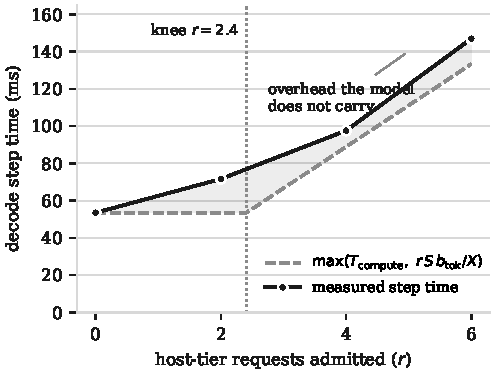
\includegraphics[width=\columnwidth]{figs/f6.pdf}
\caption{The cost of a host-tier request is not affine. Below the knee the
aggregate transfer still fits inside a step and is imperfectly hidden; above it
the step \emph{is} the transfer and each request costs its full link time. The
shaded area is overhead the kink model does not carry --- roughly 13\,ms on a
53\,ms step at the knee, which is more than two extra requests buy. A faster
interconnect moves the knee right; it does not shrink the shaded area.
Qwen2.5-32B, 2048 context, 16 device-tier residents, A100/PCIe at a measured
25.1\,GB/s, 3 repeats with under 1\% spread.}
% src: paper/data/rider_cost_phase0.json @ fb7e9db2a
\label{fig:costcurve}
\end{figure}

Two properties of the cost curve matter for the coherent-link projection. It is
\textbf{not affine}: extending the sweep, $\Delta T$ per rider \emph{rises}
($9.1$, $11.0$, $15.6$\,ms at $r = 2, 4, 6$; Fig.~\ref{fig:costcurve}), so
$\Delta T = F + cr$ fits a
negative fixed cost and the fixed-versus-slope split above is not a meaningful
decomposition. What the data fits is a kink, $T \approx \max(T_{\mathrm{compute}},
r S \btok{}/\Xlink) + \text{overhead}$, with the knee at
$r = T_{\mathrm{compute}}\Xlink/(S \btok{})$ --- $2.4$ riders here,
which is where the byte budget of \S\ref{sec:design:admission} also lands. A
faster link raises the knee but does not remove the overhead, and at the knee
$\sim\!13$\,ms of overhead on a $53$\,ms step already exceeds what two extra
requests buy. Whether that overhead survives onto a coherent interconnect is
the question the next substrate has to answer, and it cannot be extrapolated
from this one.
% src: paper/data/rider_cost_phase0.json @ fb7e9db2a

\paragraph{Swap semantics versus streaming.} A design whose offloaded unit is
\emph{owned} by one side must write that unit back once per generated token; one
whose device-side copy is a \emph{cache} need not (\S\ref{sec:related}). We
measure the difference directly by writing each layer's slot back to the host
mirror with the policy otherwise unchanged. The emulation is exact in extent:
both arms read the same $602$\,MB, and the write-back arm moves
\textbf{$2.00\times$} the total link traffic, with token output verified
identical. We report this as a mechanism check rather than a performance
result: it is measured on Qwen2.5-0.5B at $512$ context, a configuration small
enough that the ratio isolates the write-back leg without the step-time effects
that dominate at the primary model's scale.
% src: paper/data/ablation_swapback_20260911.json @ 74a5d9c58

\subsection{Does the capacity model predict it?}
\label{sec:eval:model}

Two parameters of Eq.~\ref{eq:step} are re-measured on each platform: the
weight-read efficiency $\effw$ and the paged-KV read efficiency $\effkv$ against
working-set size. The second is the larger risk to our own projections and we
run it early for that reason --- $\effkv$ sits in the capacity denominator, so a
kernel generation that reads paged KV more efficiently shortens the step,
shrinks the transfer budget, and \emph{lowers} the predicted gain.

\textbf{Neither factor of the multiplier is yet measured, and we say so.} The
multiplier has two: a bandwidth ratio $\Xlink/\BW$ and an amplifier
$\HBM/\Ckv$. Testing the first needs two interconnect generations and we have
one; testing the second needs one model at two weight precisions, which we have
not run. What this section does establish is narrower and worth separating from
the multiplier: the step-time model of Eq.~\ref{eq:step} holds across 54
configurations, the mechanism is additive, and the cost of a host-tier request
is decomposed on the substrate we have. The multiplier itself rests on that
parameter fit plus the model's agreement with a published system's results
(\S\ref{sec:model:directkv}), and a reader who discounts both should read
Table~\ref{tab:gain} as a prediction awaiting its experiment.

\subsection{When does it not pay?}
\label{sec:eval:negative}

\emph{Below the applicability gate.} Eq.~\ref{eq:gate} predicts no benefit when
the latency target is tighter than the full-pool step time; the tightest points
of the goodput sweep test that directly.

\emph{When the weights are small.} Llama-3.1-8B leaves 75.9\,GB of a 96\,GB
part after weights, so $\HBM/\Ckv = 1.26$ and the capacity multiplier is only
$\times$1.22 in capacity. It is the second gate of \S\ref{sec:model:omits} that
makes it a predicted \emph{negative}: charging $F$ and the unhidden residual
gives $\times$0.75, and its $F^{*}$ is $-7.0$\,ms, meaning the residual alone
exceeds what its capacity buys. The prediction is therefore unusually strong ---
8B should lose on \emph{any} implementation, however cheap the fixed cost.

\emph{When the interconnect is slow.} On A100/PCIe, with real KV delivered
through the prefill handover, throughput is 2.3\% \emph{below} not offloading
at all.
% src: paper/data/pd_decode_goodput.json @ f3df05bdb
That is what the model predicts for a 25\,GB/s link, and DirectKV reaches the
same boundary from the kernel side, concluding that on PCIe theirs ``should be
viewed primarily as a capacity-extension mechanism\ldots bounded by CPU--GPU
interconnect bandwidth''. We report it as a validated negative that fixes one
end of the bandwidth axis rather than as a disappointment.

\subsection{Does a second tier raise goodput?}
\label{sec:eval:goodput}

\emph{Question.} The one an operator actually asks. \emph{Claim under test.}
That at a matched latency target the mixture serves more requests per second
than either endpoint. \emph{Prediction.} On this substrate, \textbf{no}:
charging the fixed cost and the unhidden residual of \S\ref{sec:model:omits}
makes the throughput form $\times0.86$ for our primary model even on a projected
coherent link, and worse on this one. The capacity term alone does not rescue
it: what would is $F$ falling below the $F^{*} = 4.0$\,ms that configuration can
afford.

We state the protocol here because it is the experiment the positive claim
requires and it is not yet run. Hold model, device, workload and substrate
fixed; vary only whether a second tier is used; sweep arrival rate until goodput
stops rising; report goodput at a target anchored to the baseline's own measured
full-pool step time rather than a round number, since a target below an arm's
step time is unsatisfiable by every arm and measures nothing. A target at the
baseline's floor is the one a host-tier request is \emph{least} able to meet,
because it adds per-step latency; a very loose target admits everything and
discriminates nothing; the informative regime is between them. Reporting
requires the fixed cost to be measured on the same machine, since it is what the
prediction turns on.

The PCIe half of that comparison is \S\ref{sec:eval:negative}: with real KV
through the prefill handover, throughput is $2.3\%$ below not offloading, which
is the predicted sign.

\subsection{Correctness}
\label{sec:eval:correct}

A memory system that returns different tokens is not a faster memory system. We
verify in-process that a host-tier request's attention output is bitwise
identical to the same request served resident, over 576 mixed decode
layer-steps. End to end, greedy decoding through the host path matched stock
vLLM on 6 of 6 prompts in one round and 4 of 6 in another; the divergences are
bf16 accumulation order, not placement, and Appendix~\ref{app:correct} gives the
evidence for that reading. Appendix~\ref{app:correct} gives the ladder and what each
rung rules out.

% ============================================================================
% Section 7 -- related work. Claim C4 and the novelty argument.
%
% STATUS: first full draft, 2026-09-05. Survives every branch of the GH200 gate.
% Source: seven papers read end-to-end 2026-08-10; positioning table in
% paper/PAPER_OUTLINE.md section 4 (that file is RETIRED as of
% 2026-09-06; the original is in git at 2bfc6ca5e).
%
% The endpoint argument is the load-bearing paragraph. Reviewers will go
% straight to "why does DirectKV not pre-empt this" -- answer it early and in
% their own words, with their own quotes.
% ============================================================================

\section{Related work}
\label{sec:related}

\paragraph{Capacity, not compute, is what binds.} A recent trace-driven study
of KV offloading finds that device memory capacity, not token budget, limits
batch size~\cite{bottlenecks}, and names scheduler improvements as future work.
That is the premise this paper builds on, and it is measured rather than
assumed.

\paragraph{Mechanisms for host-resident KV.} DirectKV~\cite{directkv}
contributes zero-copy GPU attention over CPU-resident KV on coherent
GH200/GB200 interconnects, through CPU-memory-aware tiling, warp pipelining and
kernel fusion, eliminating the GPU staging buffer entirely. It is the state of
the art in \emph{mechanism}, and it is a competing one rather than a substrate
for ours.

\textbf{The staging buffer they remove is the thing that makes hiding
possible.} Their kernel reads host memory \emph{during} the attention that
needs it, so the transfer is inside the operation rather than alongside it;
ours prefetches layer $\ell{+}1$ into a rolling device buffer while layer
$\ell$ computes. The two designs therefore trade in opposite directions. They
pay no device memory and get no overlap; we pay one $k$-window of device memory
and overlap $\effo$ of the transfer, which on PCIe we measure at $0.62$ --- a
real window, but well short of all of it. Neither dominates on paper, and
settling it needs both mechanisms on one machine, which requires their
SM90a-only kernel and is therefore future work rather than a result we report. It also means a host-tier
request cannot simply be moved onto their kernel and remain what we call a
rider: without a prefetch window there is nothing left to hide, and such a
request pays the full transfer inside its own step.\footnote{Their architecture
would admit a mixture --- their \texttt{forward\_decode} already dispatches two
attention implementations over disjoint subsets of one batch --- but the
resulting system is a third design point, selective admission \emph{without}
hiding, not ours built on theirs.}

What their \S8.1 does establish is that the policy dimension is untouched:
``DirectKV does not change scheduling, batching, or KV-management policies;
instead, it provides an efficient execution path for CPU-resident KV
blocks\ldots while leaving the scheduler, model execution graph, and frontend
API unchanged.'' Whichever mechanism proves faster, the question of \emph{how
many} requests to serve from the host is left open by it, and that is where
this paper sits.

It is also worth recording that DirectKV's own analysis agrees with our
measured PCIe result: they conclude that ``on PCIe, DirectKV should be viewed
primarily as a capacity-extension mechanism\ldots its performance advantage
remains bounded by CPU--GPU interconnect bandwidth,'' and report NVLink-C2C
reducing attention latency by up to $4.2\times$ relative to PCIe. Our
\S\ref{sec:eval} finds the same boundary from the scheduling side. Their
evaluation covers Llama-3.1-8B and OPT-13B/30B on a GH200-96, so it does not
overlap the models we evaluate, and it does not include a 70B-class
configuration --- which our capacity model identifies as the most favourable
point of all. We do not evaluate one either (\S\ref{sec:eval:setup} says why: at
a capacity-limited batch of about seven, one request is 14\% and no result could
separate an effect from a rounding artifact), so the most favourable point of
the model's own curve is measured by nobody yet.

\paragraph{The closest prior mechanism: partitioning by layer.}
Pie~\cite{pie} is the nearest neighbour of our transfer path and deserves a
precise comparison. It targets the same hardware, stages KV through GPU buffers
as we do, and prefetches per layer through a FIFO queue so that the transfer
overlaps compute --- our rolling region and its swap buffers are cousins, and it
reports up to $1.9\times$ throughput over vLLM.

\textbf{The difference is the axis of partition.} Pie relocates $m$ of a model's
$n$ \emph{layers} of KV to host memory, ``using per-layer KV cache as the basic
management unit'', and that split applies to \emph{every request identically};
its single control is a global expansion factor, tuned adaptively so that
swap time stays inside compute time. Two consequences follow directly. First,
\textbf{no request's KV is ever fully absent from the device} --- every request
retains $(n-m)/n$ of its cache in HBM, always, so there is no configuration in
which one request is entirely host-resident while its neighbours are entirely
device-resident. Second, \textbf{interconnect bandwidth is spent uniformly}: the
per-step volume is a fixed fraction of \emph{every} request's KV, whereas ours
is the KV of the requests we select, which is what makes \emph{which requests}
a decision at all.

\paragraph{Why the request axis?} The two axes are not orthogonal, and it would
be convenient but wrong to say so: a layer split and a request split spend the
\emph{same} interconnect budget, and in the fluid model of \S\ref{sec:model} a
layer split with the right $m/n$ fills both byte budgets and reaches the same
interior point. They are substitutes, and the case for the request axis has to
be made on the terms the fluid model omits.

Three of those favour it. A host-tier request holds \emph{zero} device blocks, so
admitting one requires no allocation at all and the device pool is untouched;
under a layer split every request retains $(n-m)/n$ of its cache on the device,
so capacity is freed only in proportion and never for a whole request. Movement
happens once per request, at a moment the scheduler chooses, rather than once per
layer per token --- which is what removes Pie's return leg. And only selected
requests pay link traffic, so a load spike can be absorbed by moving a few
requests rather than by degrading all of them.

One favours the layer axis, and we concede it: a layer split has no integer
quantization. It can relocate $1/n$ of a cache where we must relocate a whole
request, so at long context, where $B_{\mathrm{cap}}$ and $B_{\mathrm{off}}$ are
small integers (\S\ref{sec:model:omits}), the layer axis reaches operating points
the request axis cannot express. A system wanting both would use a request split
for capacity and a layer split for the remainder; we have not built that, and it
is the more interesting composition than the one usually asserted.

We adopt one of Pie's measurements --- Pie reports GH200 NVLink-C2C at
419\,GB/s CPU$\to$GPU and 371\,GB/s GPU$\to$CPU, an independent confirmation
that the widely quoted 900\,GB/s is a bidirectional figure and that a
host-to-device KV stream should be budgeted well below it.

FlexGen~\cite{flexgen} is the earlier generation of the same family, placing KV
across GPU, CPU and disk by a linear-programming search with compression; it is
offline-profiled rather than adaptive. Both pay the staging cost that a
zero-copy kernel removes, and neither decides a tier per request.

DAK~\cite{dak} pushes host-resident tensors to shared memory via the Tensor
Memory Accelerator (TMA) and chooses
per-\emph{operation} offload ratios by greedy search --- but takes a
\emph{global} offload ratio as an input, which is precisely the quantity a
policy has to produce.

\paragraph{Is decode serving memory-bound at all?} NanoFlow~\cite{nanoflow}
argues the opposite of \S\ref{sec:background}: that end-to-end serving is
\emph{compute}-bound for most common workloads once operations of different
resource classes are overlapped within a device, and it reports $1.91\times$ over
prior engines by doing so. The claim is not in conflict with ours, but the
boundary between them is exactly where this paper lives. NanoFlow raises
utilisation at a \emph{given} batch by filling idle units; our premise is that
the batch itself is capped by KV capacity before those units saturate. The two
compose in principle --- a larger batch gives intra-device overlap more to work
with --- and they collide in practice if the arithmetic recovered by overlapping
pushes the step into the compute-bound regime, because then admitting a
host-tier request no longer buys throughput. Appendix~\ref{app:params} gives our own
measurement of the margin: at batch 142 for an 8B model at 4K --- far above the
capacity limit on any device we consider --- decode-attention's arithmetic
intensity has crossed the hardware balance point, yet the step is still
memory-bound by roughly $4\times$ ($30.7$\,ms of memory time against $7.4$ of
compute). So the two premises are not in conflict at the batch sizes a capacity
limit permits. On a device where that margin closes, NanoFlow's premise holds
and ours does not.

\paragraph{Moving the request instead of its memory.} Llumnix~\cite{llumnix}
reschedules requests \emph{across} model instances by live-migrating them and
their KV, to balance load, reduce fragmentation and honour priorities. It is the
natural alternative to a second memory tier: when a request will not fit here,
one can move it to another GPU rather than move its KV to the host. The choice
between them is an economic one rather than a technical one --- migration needs
a second instance with room, which is a provisioning decision, while tiering
needs only host DRAM, which is already installed and idle. They also compose
cleanly, since a tier decision is local and a migration decision is global, and
a scheduler holding both has a strictly larger action set than one holding
either. We do not evaluate that combination.

\paragraph{Architectures that shrink the cache.} The gate of
\S\ref{sec:model:gate} opens when weights consume enough of the device that
little is left for KV. Architectural changes to attention move that boundary
directly. Multi-head latent attention~\cite{deepseekv2} compresses $K$ and $V$
into a low-rank latent, cutting KV bytes per token by roughly an order of
magnitude, and sliding-window and hybrid-attention designs bound the cache by
construction rather than by context. By Eq.~\ref{eq:cancel} a uniform reduction
in $\btok$ scales both cohorts and leaves their ratio unchanged --- so shrinking
KV does not by itself close the gate. What closes it is the \emph{second} gate:
a smaller cache raises $B_{\mathrm{cap}}$, so the fixed per-step cost is
amortised over more requests but the capacity gain it must beat is unchanged in
ratio and smaller in absolute requests. We regard a serving stack built entirely
on MLA-class models as outside the regime this paper addresses, and say so
rather than claim the technique is architecture-neutral.

\paragraph{Moving compute instead of data.} NEO~\cite{neo} offloads attention
\emph{compute} to the CPU to grow the batch --- the same problem statement as
ours with the opposite mechanism. Its own scaling is the argument against it:
gains decay from $7.5\times$ on a T4 to 14\% on an H100, because a faster GPU
makes the CPU's arithmetic relatively worse. Streaming KV to the GPU depends on
a different ratio, $\Xlink/\BW$, and it would be convenient but dishonest to
present that as simply improving with hardware. Across a generation, HBM
bandwidth and capacity have both grown faster than host-to-device bandwidth, so
$\Xlink/\BW$ falls and $\HBM/\Ckv$ falls with the extra capacity --- both
factors of Eq.~\ref{eq:gain} trend \emph{against} us, which is the same
structural decay we note in NEO. What would reverse it is a link that scales
with HBM rather than with PCIe generations, which is precisely the bet a
coherent interconnect represents. \S\ref{sec:discussion} states our own
anti-scaling in the same terms.

\paragraph{Summary of the gap.} Table~\ref{tab:axes} places the systems that
share our hardware assumption on the two questions that matter: what unit of KV
is placed, and who decides.

\begin{table}[t]
\centering
\small
\begin{tabular}{llll}
\toprule
 & placement unit & decided by & device KV \\
\midrule
vLLM, SGLang & --- & --- & all of it \\
Pie~\cite{pie} & layer, uniform & global factor & $(n{-}m)/n$ each \\
DirectKV~\cite{directkv} & none (all host) & nothing & none \\
\textbf{this paper} & \textbf{request} & \textbf{placement,} & resident \\
 & & \textbf{admission,} & cohort \\
 & & \textbf{migration} & only \\
\bottomrule
\end{tabular}
\caption{The mechanism for reading host-resident KV efficiently is solved; the
open question is which requests should live where. Systems either place nothing
(both endpoints) or place a fixed fraction of everything (Pie), and none decides
per request.}
\label{tab:axes}
\end{table}

What is unsolved is which requests should live in which tier, how many host-tier
requests a step can absorb without breaking the resident cohort's latency, and
when a request should move. DirectKV~\cite{directkv} states it explicitly
(\S8.1: the design ``does not change scheduling, batching, or KV-management
policies''), Fang et al.~\cite{calkv} close by calling for runtime policies, and
OmniServe~\cite{omniserve} takes its service classes as externally supplied
rather than inferring them.

% PROVENANCE: this section derives from \S\ref{sec:model} and \S\ref{sec:eval} and
% introduces no new measurements; where it quotes a number it points at the section
% that sourced it.
%
% CUT TO ~0.7pp 2026-09-27. The four subsections are now two plus limitations. The
% expanded forms -- composition with orthogonal techniques, the third-tier
% structure, the per-limitation detail -- are in appendix F.
\section{Discussion}
\label{sec:discussion}

\subsection{The window is a result, and it is shrinking}

Eq.~\ref{eq:gate} and Eq.~\ref{eq:gain-exact} together form a deployment rule that
can be evaluated before building anything: a second KV tier pays when the latency
target exceeds the full-pool step time plus $F$, and it pays in proportion to
$\HBM/\Ckv$. Both exclude configurations the field routinely evaluates on. We state
the window as a finding rather than a caveat because the alternative is worse --- a
technique whose applicability is unstated gets evaluated where it happens to win.

The gain also \textbf{shrinks as device memory grows}, and for our primary model it
does not merely shrink: Qwen2.5-32B on a 144\,GB device leaves $\Ckv \approx
71$\,GB, at which point the gate stops admitting at all. Both factors of
Eq.~\ref{eq:gain-exact} trend that way across a hardware generation, since HBM
bandwidth and capacity have grown faster than host-to-device bandwidth --- the same
structural decay we identify in compute-offload systems (\S\ref{sec:related}), and
it would be dishonest to cite that against them without stating it about ourselves.
Model growth bears the other way: 405B-class models push $\HBM/\Ckv$ up, so the
favourable configurations are becoming more common even as each device generation
makes them rarer. Weight \emph{precision} cuts against us for the same reason ---
quantizing weights returns memory to $\Ckv$ and removes the amplifier, where
quantizing KV scales both cohorts and leaves their ratio unchanged, so a memory
system and a precision decision are not independent.

Nothing in the design is specific to host DRAM or to one attention kernel --- what
it asks of a tier is the three properties of \S\ref{sec:background}, and moving
platform means re-measuring five quantities: the two read bandwidths, the link, and
the host path's fixed and per-request costs. Appendix~\ref{app:coherence} works
that through, with the third-tier structure and the staging-versus-zero-copy
crossover.

\paragraph{Limitations.} Four bound the result and
Appendix~\ref{app:coherence} gives each in full: the evaluation is one device on the
wrong link, so every positive claim is marked a prediction; the model assumes dense
GQA attention and uniform context, so it covers neither MoE nor MLA-class models and
charges nothing for host DRAM bandwidth; the regime is real but not universal, since
an operator whose weights fill the device can also quantize them or add a GPU; and
the headline is bounded by an engineering number, since $F$ is a property of the
current design rather than a tuned result. That last bound is now quantified rather
than open: $F$ is down $74\%$, and both halves of what remains are priced by
ablation. Fusing the two attention calls is worth $+2$ to $+8.5$ points --- a range
rather than a number, because the part that certainly goes is per-rider gather work
while the rest is a kernel whose arithmetic survives fusion --- and the mirror
write's remainder is bounded below by $0.83$\,ms of unavoidable copies
(Appendix~\ref{app:ridercost}). The prefill transport is also emulated
(\S\ref{sec:impl:stash}).


\bibliographystyle{plain}
\bibliography{refs}

% MLSys allows unlimited appendices; reviewers are not required to read them.
% What lives here is material a reader may want to check but does not need in
% order to follow the argument: parameter measurement, implementation detail,
% and the correctness ladder.
\appendix
% Appendix A -- parameter measurement, moved out of section 3 (2026-09-26) to
% keep the body within the MLSys page limit. Nothing here is needed to follow
% the argument; all of it is needed to check it.

\section{Measured parameters and sensitivity}
\label{app:params}

A100-80 PCIe; two models; 41 single-shot configurations plus a
13-configuration $n{=}3$ repeat sweep; distinct random contexts; prefix caching
disabled.
% src: paper/model/p4_llama8b_a100_rep3.json @ 2bfc6ca5e

\paragraph{Weight read is efficient and stable within a model.} $\effw \approx
0.75$ of the measured $1935$\,GB/s peak ($\approx$1450\,GB/s achieved). The
$B{=}1$ steps must have their KV term subtracted before $\effw$ is read off
them: it is 1.6\% of the step at 2K context and 6.0\% at 8K, and leaving it in
manufactures a drift (0.729 falling to 0.694 for Llama-3.1-8B) that is the KV
term growing rather than the weight read degrading. Subtracted, $\effw$ is
0.741/0.736/0.738 for Llama-3.1-8B across 2K--8K and 0.778/0.777 for
Qwen2.5-32B --- flat within each model, and 5.3\% apart between them. We carry
the single value 0.75, which is between them, and \S\ref{sec:model:cancel}
reports what each choice predicts.

\paragraph{Paged KV read is neither.} $\effkv$ degrades by $1.6\times$ with the
KV working set (Table~\ref{tab:effkv}):

\begin{table*}[t]
\centering
\small
\begin{tabular}{lrrrrr}
\toprule
KV working set & 4.3\,GB & 8.6\,GB & 17--34\,GB & 43\,GB & 51.5\,GB \\
\midrule
$\effkv$ & 0.77 & 0.72 & 0.54--0.56 & 0.49 & 0.46 \\
\bottomrule
\end{tabular}
\caption{Paged KV read efficiency is not a constant. Error bars from $n{=}3$
repeats are $\pm0.02$--$0.04$; the degradation is far outside them. The
17--34\,GB column takes 0.55 rather than the 0.747 measured at
$B{=}16,S{=}8192$ --- the anomaly discussed below. That is the
\emph{optimistic} choice for us, since a lower $\effkv$ lengthens the step and
so raises the projected gain, and we note it rather than let it pass.}
\label{tab:effkv}
\end{table*}

This is the real correction to the model. It also bears on how such models are
built elsewhere: \textbf{a roofline that charges KV at one fixed bandwidth will
be optimistic at the capacity-bound operating point}, because that is where
$\effkv$ is worst. We measured this on one GPU and one kernel generation
(A100, FlashAttention-2 era), so we state it as a property of what we measured
rather than of the literature.

\paragraph{A caveat at kernel granularity.} The claim that only total KV bytes
matter holds at three of four same-byte test points but breaks at 17.2\,GB
($B{=}32,S{=}4096$ gives 0.561 against $B{=}16,S{=}8192$ at 0.747). The cause
is a reproducible anomaly at $B{=}32,S{=}4096$ that also appeared in an
independent earlier run --- an attention-kernel scheduling artifact, most
likely a split-KV heuristic in the attention kernel choosing a different
partitioning at the larger batch, not measurement noise ($\pm0.61$\,ms
against a $\sim$3\,ms deviation). The aggregate law holds; the
per-configuration surface has kernel-regime steps.

\paragraph{Compute is not the binding term.} Decode-attention arithmetic
intensity equals the GQA group size --- 8 for 70B, 4 for 8B --- against an
H100 balance point near 116 FLOP/byte, so attention sits 14--29$\times$ below
the compute roof. At batch 8, 70B spends 7\% of its step on arithmetic.
% src: paper/model/compute_check.py @ 2bfc6ca5e
Llama-8B at 4K crosses the arithmetic-intensity balance point at batch 142, while its step remains memory-bound by about $4\times$, which is a further
reason it is the wrong model to evaluate on.


% Appendix B -- the correctness ladder, moved out of section 6 (2026-09-26) for
% the page limit. A reviewer who doubts the mechanism should read this; one who
% doubts the economics should not need to.

\section{Correctness ladder}
\label{app:correct}

Placement moves bytes rather than approximating them, so these gates are
hygiene rather than a contribution. Numerically we verify the host pool's round
trip, the two-tier attention against a single-pass reference over the same KV
(576 mixed decode layer-steps, $\max|\mathrm{diff}| = 0$), and the prefill
handover across block boundaries and after the producer's memory has been
recycled. End to end we compare generated tokens against stock vLLM.

One methodological note, because it traps anyone reproducing this.
\texttt{bf16} attention reductions are not associative, so their result depends
on batch composition: stock vLLM produces different text for the same prompt at
concurrency 1 and at 6, reproducibly at each. Any system that changes batching
--- as a memory tier does --- will diverge on such prompts without being wrong.
We therefore compare serially, batch of one on both sides, and under load only
on prompts pre-screened as batching-stable. For calibration: on a serial greedy
comparison our host tier matched stock vLLM on 6 of 6 prompts in one round and
4 of 6 in another, while enabling \emph{vLLM's own prefix cache} --- changing
nothing else --- matched on 2 of 6.

% Appendix C -- the detailed adjudication of related work, moved out of
% section 7 (2026-09-26) for the page limit. The body keeps every claim this
% paper's positioning rests on; what is here is the evidence for those claims,
% which a reviewer checking our reading of another paper will want and a reader
% following the argument will not.

\section{Related work in detail}
\label{app:related}

\paragraph{Where Pie's advantage comes from, and where it stops.} Pie's
headline is $1.9\times$ over vLLM, and the regime that produces it is stated
plainly in their \S5.3: they hold the physical KV cache fixed and sweep it from
3 to 12\,GB, and report that Pie ``outperforms vLLM at smaller GPU KV cache
sizes and achieve similar performance at the largest memory capacity
(12\,GB)'', because ``when GPU memory capacity is small, vLLM suffers from
significant recomputation''. As memory grows, ``the improvement ratio gradually
decreases until Pie and vLLM perform similarly''.

The gain is therefore \emph{avoided recomputation} in a memory-starved engine,
not additional capacity converted into work. That distinction matters for what
each system can claim. A device large enough that the baseline stops preempting
is a device on which Pie's reported advantage has already converged to zero ---
and their entire sweep, 3 to 12\,GB of KV, sits below the operating point we
study, where a 32B model on a 96\,GB device leaves $\Ckv \approx 22$--28\,GB.

\paragraph{A consequence of the layer unit: the return leg.} Choosing the layer
as the unit of management has a second effect, on traffic rather than on
policy. In Pie a layer's KV \emph{lives} on one side or the other, and the
GPU-side buffer it occupies is needed by the next layer arriving, so a layer
that has just been computed --- and has therefore just had this token's $K,V$
appended to it --- must be written back in full. Their swap controller says so
directly: it initiates ``a swap-out for the `coldest layer', defined as the last
layer that finished computation''. Every offloaded byte therefore crosses the
interconnect \textbf{twice per generated token}, and the return leg is the
slower direction (371 vs 419\,GB/s by their own measurement).

Our rolling region is not the home of the data but a cache of it: the host
mirror stays authoritative and each step's new $K,V$ is written to it directly,
so a slot can be overwritten without persisting anything. DirectKV's kernel has
the same property, appending only the newly projected $K,V$ to CPU memory. The
resulting difference in per-token traffic is not marginal:

\begin{table}[t]
\centering
\small
\begin{tabular}{lll}
\toprule
per generated token & to device & to host \\
\midrule
Pie~\cite{pie} & offloaded KV & \textbf{the same KV again} \\
DirectKV~\cite{directkv} & all KV & one token's $K,V$ \\
\textbf{this paper} & selected requests' KV & one token's $K,V$ \\
\bottomrule
\end{tabular}
\caption{Per byte of offloaded KV, a design whose offloaded unit is \emph{owned}
by one side must return it; one whose device-side copy is a \emph{cache} need
not. Pie moves two bytes where the other two move one, and its return leg uses
the slower direction of the link.}
\label{tab:traffic}
\end{table}

Table~\ref{tab:traffic} states the consequence. This is not a criticism of
Pie's design so much as a property of its unit:
a whole layer's cache cannot be left dirty on the device when the buffer is
reclaimed for the next layer. It does mean that comparisons of interconnect
pressure between these systems must count both directions.

\paragraph{On comparing directly.} Pie has no public artifact --- its paper
lists no repository, and we found none --- so a head-to-head against their
implementation is not available to us. Nor would it isolate what we want:
running two engines compares implementations, whereas the question here is
whether \emph{choosing} which requests to offload beats spreading the same
interconnect budget uniformly. \S\ref{sec:eval:ablation} therefore holds the
mechanism fixed and varies the policy, and reports Pie's published figures
alongside rather than reproducing them.


\paragraph{The endpoint argument.} DirectKV \S6: ``During prefill, the manager
stores the initial $K,V$ entries from each layer in CPU memory. During decode,
the GPU reuses these cached entries directly, while only appending new $K,V$
for the latest token'' --- and its Alg.~3 appends that new $K,V$ to CPU memory
as well. \textbf{It places 100\% of KV on the host, for every request, always.}
That is why it needs no scheduler: placement is static and total. Stock vLLM
and SGLang are the opposite endpoint, at 0\%. Pie is the one system that is
genuinely interior, and it reaches the interior by splitting \emph{layers}
uniformly across all requests rather than by choosing requests --- so the
per-request axis is unoccupied, and the optimum along it is interior
(Table~\ref{tab:endpoints}). Note that the all-host endpoint leaves the device
memory not holding weights entirely idle, which is why it loses to an
HBM-resident baseline whenever that baseline fits --- the ordering DirectKV
reports on Llama-3.1-8B, and one our gain law is consistent with
(\S\ref{sec:model:directkv}).

A natural objection to reading DirectKV \S8.1 as leaving the policy dimension
open is that the vLLM and SGLang mechanisms it names --- continuous batching,
prefix reuse, eviction, hierarchical KV caching --- already constitute KV
policy. They do not, for our purposes: each decides \emph{reuse} and
\emph{preemption}, that is, the residency of blocks belonging to a request that
is \emph{not currently decoding}. None of them decides the tier of an
\emph{actively decoding} request. Several systems do \emph{decode} from
host-resident KV --- FlexGen, Pie, NEO and OmniServe among them --- so the state
is not new; what is unoccupied is choosing, per request, which side of the
memory such a request lives on.

\paragraph{Policy, at other granularities.} OmniServe~\cite{omniserve} is the
closest prior work on policy: it forms mixed GPU/host batches and admits
host-tier work per layer under an SLO. The regime differs on three axes that
change the problem. It targets PCIe-attached A100s with CPU-only hosts over
RoCE; attention for host-tier requests is computed \emph{on the CPU}, so the
trade is compute-for-capacity rather than bandwidth-for-capacity; and tiering
is driven by an \emph{externally supplied} latency-sensitive/best-effort
service class. Ours assumes a coherent interconnect, computes all attention on
the GPU, and infers tier from observable request properties, so it applies in a
single-class deployment where no such label exists.

Fang et al.~\cite{calkv} --- whose title also claims the phrase ``heterogeneous
memory system'', so the distinction is worth drawing sharply --- give a formal
placement model and a
simulated-annealing oracle bound on aggregate bandwidth. It is simulation only,
on synthetically shrunk HBM, at \emph{token} granularity by importance, and it
requires perfect foresight; its gains are contingent on 60--80\% attention
sparsity, and it closes by explicitly calling for runtime policies. Its own
results show migration overhead dominating below roughly 60\% sparsity. We
make the testable counter-claim that \emph{request}-granularity migration
avoids that thrash, because whole requests move once at controlled moments
rather than pages chasing shifting token importance.

\paragraph{Reducing the KV instead of relocating it.} ShadowKV~\cite{shadowkv}
keeps a low-rank $K$ on the GPU, offloads $V$, and reconstructs sparsely,
reporting support for a $6\times$ larger batch and $3.04\times$ throughput; KV
quantization, Quest and H2O likewise shrink what must be stored. These change
the model's output, and they compose with a memory system rather than competing
with it: a smaller KV scales both the device-resident cohort and the affordable
host cohort, leaving the ratio between them --- and hence the value of a second
tier --- unchanged. That argument is analytical and we have not measured the
composition; it is a prediction of Eq.~\ref{eq:cancel}, and a cheap one to
falsify.


\paragraph{Adjacent memory management.}
InfiniGen~\cite{infinigen} attacks the same per-step transfer from the other
end, speculating which tokens matter for the next layer and prefetching only
those; it reduces the bytes a host-tier request must move, where we decide how
many requests move bytes at all, and the two are complementary.
CachedAttention~\cite{cachedattention} keeps the KV of \emph{inactive}
conversation sessions in a hierarchical store so a later turn skips prefill ---
the case \S\ref{sec:background} distinguishes from ours, and the reason our
novelty claim is scoped to actively decoding requests rather than to
host-resident KV in general. vAttention~\cite{vattention} changes how KV is
\emph{allocated}, decoupling virtual from physical memory instead of paging in
user space; it is orthogonal to placement, and a host tier built on it would
face the same admission question we pose here.



\subsection*{Composition with a zero-copy kernel}

\textbf{The staging buffer they remove is the thing that makes hiding
possible.} Their kernel reads host memory \emph{during} the attention that
needs it, so the transfer is inside the operation rather than alongside it;
ours prefetches layer $\ell{+}1$ into a rolling device buffer while layer
$\ell$ computes. The two designs therefore trade in opposite directions. They
pay no device memory and get no overlap; we pay one $k$-window of device memory
and overlap $\effo$ of the transfer, which on PCIe we measure at $0.62$ --- a
real window, but well short of all of it. Neither dominates on paper, and
settling it needs both mechanisms on one machine, which requires their
SM90a-only kernel and is therefore future work rather than a result we report. It also means a host-tier
request cannot simply be moved onto their kernel and remain what we call a
rider: without a prefetch window there is nothing left to hide, and such a
request pays the full transfer inside its own step.\footnote{Their architecture
would admit a mixture --- their \texttt{forward\_decode} already dispatches two
attention implementations over disjoint subsets of one batch --- but the
resulting system is a third design point, selective admission \emph{without}
hiding, not ours built on theirs.}

What their \S8.1 does establish is that the policy dimension is untouched:
``DirectKV does not change scheduling, batching, or KV-management policies;
instead, it provides an efficient execution path for CPU-resident KV
blocks\ldots while leaving the scheduler, model execution graph, and frontend
API unchanged.'' Whichever mechanism proves faster, the question of \emph{how
many} requests to serve from the host is left open by it, and that is where
this paper sits.

It is also worth recording that DirectKV's own analysis agrees with our
measured PCIe result: they conclude that ``on PCIe, DirectKV should be viewed
primarily as a capacity-extension mechanism\ldots its performance advantage
remains bounded by CPU--GPU interconnect bandwidth,'' and report NVLink-C2C
reducing attention latency by up to $4.2\times$ relative to PCIe. Our
\S\ref{sec:eval} finds the same boundary from the scheduling side. Their
evaluation covers Llama-3.1-8B and OPT-13B/30B on a GH200-96, so it does not
overlap the models we evaluate, and it does not include a 70B-class
configuration --- which our capacity model identifies as the most favourable
point of all. We do not evaluate one either (\S\ref{sec:eval:setup} says why: at
a capacity-limited batch of about seven, one request is 14\% and no result could
separate an effect from a rounding artifact), so the most favourable point of
the model's own curve is measured by nobody yet.

% Appendix D -- two design figures moved out of section 4 (2026-09-26) for the
% page limit. Both illustrate structure the body states in prose; the three that
% stayed (the per-layer execution split, the compaction, and the k-slot
% pipeline) show things prose cannot.

\section{Additional design figures}
\label{app:figures}

\begin{figure*}[t]
\centering
\begin{tikzpicture}[
  x=1cm, y=1cm, font=\small,
  box/.style={draw, rounded corners=2pt, align=center, inner sep=2mm},
  mem/.style={box, fill=black!4},
  hot/.style={box, fill=blue!8, draw=blue!45},
  lbl/.style={font=\scriptsize\itshape, text=black!60, align=center},
  arr/.style={-{Latex[length=2mm]}, thick},
]
\node[mem, minimum width=3.2cm] (hk) at (0,0)
     {\texttt{host\_k}[$\ell$]\ \ \texttt{host\_v}[$\ell$]};
\node[lbl] (hkl) at (0,-0.85) {one pinned pair per layer,\\block-major, addressed by\\\textbf{host block id}};
\node[draw, dashed, rounded corners=3pt, fit=(hk)(hkl), inner sep=2.5mm] (hostbox) {};
\node[font=\bfseries\small] at (0,1.15) {Host DRAM};

\node[mem, minimum width=3.6cm] (pool) at (8.0,0.95)
     {paged KV pool\\[-1pt]{\scriptsize device-tier requests}};
\node[hot, minimum width=3.6cm] (roll) at (8.0,-0.95)
     {rolling region\\[-1pt]{\scriptsize $k$ slots $\times\ R$ blocks}\\[-1pt]{\scriptsize layer $\ell$ uses $\ell \bmod k$}};
\node[draw, dashed, rounded corners=3pt, fit=(pool)(roll), inner sep=2.5mm] (devbox) {};
\node[font=\bfseries\small] at (8.0,2.3) {GPU HBM};

\node[box, minimum width=2.5cm] (attn) at (14.0,0)
     {attention\\layer $\ell$\\[-1pt]{\scriptsize one forward pass}};

\draw[arr, blue!65] (hostbox.east|-hk) -- (4.4,0) -- (4.4,-0.95) -- (roll.west);
\node[lbl, text=blue!70] at (3.3,1.15)
     {\texttt{stream\_layer}($\ell$)\\refresh slot $\ell \bmod k$\\contiguous runs, H2D};

\draw[arr, black!60] (pool.east) -- (11.6,0.95) -- (attn.north west);
\node[lbl] at (11.55,1.55) {device\\block table};

\draw[arr, black!60] (roll.east) -- (11.6,-0.95) -- (attn.south west);
\node[lbl] at (11.55,-1.55) {compacted\\block table};

\draw[arr, red!60] (attn.south) -- (14.0,-2.9) -- (0,-2.9) -- (hostbox.south);
\node[lbl, text=red!70] at (7.0,-3.25)
     {\texttt{write\_token}($\ell$): this step's new $K,V$ $\rightarrow$ host mirror (authoritative) \emph{and} the current slot};
\end{tikzpicture}
\caption{\textbf{Data path.} A host-tier request's KV lives in per-layer pinned
host mirrors addressed by an independent \emph{host block id} space. Once per
step the active cohort's blocks are compacted into a rolling region of $k$
device slots (Fig.~\ref{fig:compact}); once per layer the slot for
$\ell \bmod k$ is refreshed (Fig.~\ref{fig:pipeline}). Attention runs over both
tiers in one forward pass, each tier reading its own block table.}
\label{fig:arch}
\end{figure*}

\begin{figure}[t]
\centering
\resizebox{\columnwidth}{!}{%
\begin{tikzpicture}[
  x=1cm, y=1cm, font=\scriptsize,
  st/.style={draw, rounded corners=2pt, align=center, minimum height=7.5mm,
             minimum width=1.95cm, inner sep=1.2mm, fill=black!3},
  hs/.style={st, fill=blue!10, draw=blue!45},
  arr/.style={-{Latex[length=1.5mm]}},
  ed/.style={font=\scriptsize\itshape, text=black!60, align=center},
]
\node[st] (wait) at (0,0) {waiting};
\node[hs] (adm)  at (2.9,1.35) {admitted host-tier\\{\scriptsize 0 device blocks}};
\node[hs] (dec)  at (6.0,1.35) {decoding\\host-tier};
\node[st] (res)  at (6.0,-1.35) {decoding\\device-tier};
\node[st] (fin)  at (9.6,0) {finished};

\draw[arr] (wait) -- node[ed, above, sloped] {tier $=$ host} (adm);
\draw[arr] (wait) -- node[ed, below, sloped] {tier $=$ device} (res);
\draw[arr] (adm)  -- node[ed, above, align=center] {\textbf{worker ack}\\KV present} (dec);
\draw[arr] (dec)  -- node[ed, above, sloped] {done} (fin);
\draw[arr] (res)  -- node[ed, below, sloped] {done} (fin);

% migration: two vertical arrows, separated so their labels never meet
\draw[arr] ([xshift=-7mm]res.north) -- ([xshift=-7mm]dec.south);
\node[ed, anchor=east, align=right] at (5.15,0)
     {\textbf{demote}\\on seed ack:\\release blocks};
\draw[arr, dashed] ([xshift=7mm]dec.south) -- ([xshift=7mm]res.north);
\node[ed, anchor=west, align=left] at (6.85,0)
     {\textbf{promote}\\atomic refill};
\end{tikzpicture}}
\caption{\textbf{Request lifecycle.} A request admitted directly to the host
tier never allocates a device block. A resident request that is demoted releases
its blocks only after the worker acknowledges that its KV reached the host ---
releasing on the assumption that it did would destroy the request's history.
Promotion refills the block list atomically; a partial refill is treated as a
failed promotion and the request stays on the host tier.}
\label{fig:lifecycle}
\end{figure}
% Appendix E -- the engineering lessons behind the 37.0 -> 12.3 ms reduction,
% moved out of section 5 (2026-09-26) for the page limit. The body keeps the
% number the model uses and what it is made of; this is how it got there, which
% is useful to someone rebuilding the path and not to someone reading the
% argument.

\section{Lessons from the transfer path}
\label{app:impl}

Beyond the transfer itself, using the host path costs a fixed \textbf{12.3\,ms}
per step, reduced from 37.0. That residual is the $F$ of
\S\ref{sec:model:omits}, on which the paper's result turns, so how it was found
and what it is made of both matter.

\paragraph{Layout decides whether the DMA engine can do the gather.} The mirrors
are block-major with $K$ and $V$ in separate tensors, so a run of consecutive
host blocks is one contiguous byte range on both sides and a layer's transfer is
a few \texttt{cudaMemcpyAsync} calls from pinned memory. An earlier layout
interleaved $K$ and $V$, making a run two chunks strided by a whole plane: no
pinned DMA was possible, and the resulting host-side gather cost 22\,ms per
layer, 98\% of the streaming path. The general point is that this cost is
invisible to the metric one would naturally watch, because it is a \emph{host}
memcpy that a faster interconnect does not touch --- on a coherent link the same
code would spend hundreds of milliseconds per step gathering in order to hide a
transfer of a few, and the natural conclusion would have been that the
interconnect does not help.

\paragraph{Hoist schedule-invariant work out of the per-layer path.} Four sites
executed work inside the per-layer loop that is fixed once the step's schedule is
known: a device reduction and a \texttt{.item()} inside a guard whose purpose was
to \emph{skip} work, scatter indices rebuilt per layer, a sequence maximum and an
\texttt{arange}, and a clone and index-fill of the masked sequence lengths.
Together they were worth 21\,ms per step, moving the end-to-end throughput
deficit from $-11.3\%$ to $-2.3\%$.

\paragraph{Time asynchronous GPU work with operator diffs, not phase timers.}
Aggregate per-phase timers misattributed this cost twice, plausibly each time: a
timer wrapped around asynchronous work charges waiting-for-the-GPU to whichever
phase holds it, and a profiler that synchronises inside its own timing wrapper
makes double-buffering impossible by construction and then reports that
double-buffering does not help. What located all four sites was an
operator-level trace differencing a step with one host-tier request against a
step with none. The same discipline applies to absolutes: the prefill handover of \S\ref{sec:impl:stash}
first measured 4.06\,GB/s on a contended node against 38\,GB/s exclusive on an
idle one, a $9.4\times$ error from contention, which is why
\S\ref{sec:eval:setup} requires exclusive access for every absolute.

\paragraph{What the residual is made of.} An operator trace shows
\texttt{cudaStreamSynchronize} gone and no dominant remaining term: roughly 640
extra kernel launches per step, about ten across 64 layers at 0.19\,ms each,
which is 12.2\,ms --- the per-layer structure itself. Removing it needs batching
across layers rather than issuing per layer, which we have not built. It is
launch-bound rather than bandwidth-bound, so a faster interconnect does not
shrink it; but it is \emph{not} machine-independent, since launch cost depends on
the host CPU and the count scales with layer depth. Whether it is smaller on a
Grace host is the first thing \S\ref{sec:eval} must measure.

% Appendix F -- the staging/zero-copy crossover in full, moved out of section 8
% (2026-09-26) for the page limit. The body states the ordering and why each
% system is right for its own design point; this is the argument behind it.

\section{Staging versus zero-copy, in full}
\label{app:coherence}

Our host tier stages: a layer's KV is copied from a pinned host mirror into a
device rolling slot before attention reads it. DirectKV's kernel instead reads
CPU-resident KV directly, with no staging buffer. We built on a staged backend
for two practical reasons --- it runs on PCIe as well as on a coherent link,
which is what let us measure the negative regime at all, and their kernel is
SM90a-only with no build on our development hardware. Our results are therefore
\emph{conservative with respect to mechanism}: a better transfer path would
raise them.

It is still tempting to read the buffer as a tax that zero-copy removes, and
that reading is wrong in a way that decides which mechanism belongs where. The
two designs hide the transfer behind different things. A zero-copy kernel
overlaps its fetch with the arithmetic of the attention tile it is already
computing --- a window of one tile, and decode attention's intensity is the GQA
group size, 4--8 FLOP/byte against a balance point near 100, so there is almost
no arithmetic there to hide behind. Staging overlaps the fetch for layer
$\ell{+}1$ with the entire compute of layer $\ell$, including the QKV, output
and MLP projections, which are weight-bound and long --- 21 of a 34\,ms step for
Qwen2.5-32B by the projection of \S\ref{sec:model}. \textbf{The staging buffer
buys a layer-sized hiding window instead of a tile-sized one.}

What it costs is two extra HBM passes per byte and the slot's own footprint, so
the comparison is a crossover in offload ratio rather than a dominance. When the
per-step transfer fits inside the layer compute window, staging hides it and pays
only the extra HBM traffic, which at $\Xlink/\BW \approx 0.105$ is a small
fraction of something already hidden; when the transfer exceeds that window it is
exposed under either design, and zero-copy wins by avoiding the passes. This is
why the two systems make opposite choices and both are right: DirectKV places
100\% of KV on the host, so its per-step transfer is the whole working set and can
never fit a compute window, while we place a selected subset and size it to fit
by construction (\S\ref{sec:design:admission}). \textbf{The offload ratio is the
quantity our policy controls}, so the choice of mechanism follows from the policy
rather than constraining it.

A coherent link would help one cost that is not about hiding. Each step projects
new $K,V$ for every host-tier request and we copy them device-to-host to keep the
mirror authoritative; mapped host memory would let the kernel write them in
place, as DirectKV's Alg.~3 does. The saving is small in time --- an asynchronous
version measured 1.6\,ms --- but it removes a class of state rather than an
amount of time, and that state is where migration bugs live. What coherence does
not buy is a cheaper transport: it is a guarantee about visibility, and the same
bytes still cross the link at link bandwidth when the kernel touches them.


% Appendix G -- the DirectKV ordering argument in full, moved out of section 3
% (2026-09-26). The body states the account and that we hold it weakly; this is
% why, in detail. The section itself says the contribution does not rest on it,
% which is the argument for it not occupying body pages.

\section{The DirectKV ordering, in detail}
\label{app:directkv}

DirectKV~\cite{directkv} reports that on Llama-3.1-8B its zero-copy host-KV
attention is \emph{slightly slower} than the HBM-resident SGLang baseline, and
that it wins on OPT-13B and OPT-30B, where SGLang runs out of memory.

Our amplifier offers an account of the ordering. Llama-3.1-8B's 16\,GB of
weights leave $\Ckv \approx 76$\,GB of a 96\,GB part, so
$\HBM/\Ckv \approx 1.26$ and there is little to buy; any overhead the mechanism
carries then shows up as a net loss. OPT-30B's 60\,GB leave
$\Ckv \approx 32$\,GB, tripling the amplifier.

We put this no more strongly than that, for three reasons a reader will find
anyway. First, Eq.~\ref{eq:gain} compares a \emph{mixture} against all-HBM,
while DirectKV is all-host; our law does not predict that an all-host system
beats an all-HBM one, and on its own terms it predicts the opposite. Second,
their OPT wins are reported ``where SGLang OOMs'', and OPT uses multi-head
attention with several times the KV bytes per token of a GQA model --- so the
baseline may be failing because $S\btok$ is large rather than because weights
are, and those are different axes. Third, OPT-13B has $\HBM/\Ckv$ close to the
8B's and yet DirectKV wins on it, which our amplifier alone does not account
for. The honest summary is that the model is \emph{consistent with} the
direction of a two-point published ordering, which is weak evidence, and we do
not rest the contribution on it.

% Appendix H -- REWRITTEN 2026-10-06. Was "The superseded rider sweep": the
% four-point sweep set aside in 2026-09-26, kept so a reader who had met its 78%
% overlap figure could see what replaced it.
%
% That framing no longer fits, because the thing that replaced it has itself been
% replaced. The four-point sweep was not merely imprecise, it was fitted ACROSS the
% knee, and so was its successor. This appendix now carries the characterisation
% done below the knee, the coefficient table with provenance, and the full ledger
% of optimisations attempted -- including the ones that failed, which is the part
% a reader extending this work most needs.
%
% The long-form version, with every arm and every retraction, is
% paper/OVERHEAD_CHARACTERISATION.md in the repository; it is not part of the
% paper.

\section{The overhead law, measured}
\label{app:ridercost}

\subsection{Why the earlier fits were wrong, and in which direction}

Three successive readings of the per-rider cost appear in this project's history,
and all three errors have one cause: \textbf{points above the knee were included in
the fit}. Above $r^{*}$ (Eq.~\ref{eq:knee}) the step time \emph{is} the transfer, so
it grows with $r$ at the link rate rather than at the overhead rate. A line fitted
through points on both sides of the boundary therefore tilts --- it borrows slope
from the transfer-bound regime and pays for it with a depressed intercept.

That single mechanism explains every discrepancy we chased:

\begin{itemize}\itemsep1pt \parskip0pt
\item the per-rider cost came out $2.2$--$2.9$\,ms, against $0.52$ measured below
  the knee: \textbf{over} by four to five times;
\item the fixed cost came out $9.6$--$12.3$\,ms, against $3.4$: \textbf{under},
  once the optimisations below are also accounted for;
\item an apparent \emph{negative} fixed cost at one configuration, which we
  reported as evidence that the law was not affine;
\item an apparent dependence of the per-rider cost on context,
  $c = 0.205 + 1.84\times10^{-3}S$, which vanishes entirely below the knee;
\item an apparent $62\%$, later $88\%$, transfer-overlap efficiency --- a quantity
  that does not exist, since below the knee the overlap is complete.
\end{itemize}

The lesson is procedural rather than numerical. The knee must be computed
\emph{per point} from the final sequence length, not the prompt length, and points
failing $\ell/T_0 \le 1/3$ must be discarded rather than down-weighted. Doing that
is what makes the two coefficients separately identifiable: across seven arms the
per-rider cost repeats to $1.5\%$ and the fixed cost to $10\%$ between runs of one
configuration.

\subsection{The coefficients}

\begin{center}\small
\begin{tabular}{llr}
\toprule
Quantity & Value & Provenance \\
\midrule
$c$ intercept       & $0.177$\,ms            & $L = 16, 32, 64$ at ctx 128 \\
$c$ per layer       & $0.0054$\,ms           & same \\
$F$ per layer       & $0.053$\,ms            & after T1, T2, T7a, T8 \\
mirror write        & $1.2$--$1.5$\,ms       & ablation at $L = 64$ \\
second attention    & $1.9$\,ms              & ablation at $L = 64$ \\
D2H copy floor      & $0.834$\,ms            & off-engine, $2L$ copies \\
\bottomrule
\end{tabular}
\end{center}
% src: paper/data/overhead/15_clean_cf/CF_L16.json,
% paper/data/overhead/15_clean_cf/CF_L32.json,
% paper/data/overhead/15_clean_cf/CF_c128_a.json,
% paper/data/overhead/20_f_split_post_t8/FS_nod2h.json,
% paper/data/overhead/20_f_split_post_t8/FS_both.json

Two cautions. The fixed cost's run-to-run drift on identical configuration was
$0.04$, $0.43$, $0.04$ and $0.51$\,ms across four jobs --- \textbf{bimodal}, so a
tight bracket in one job licenses nothing about another; we quote $\pm 0.5$\,ms and
re-measure the baseline inside every job. And the two components of $F$ are each a
single arm, so they are $\pm 0.5$ individually while their sum is pinned by the
tighter three-arm baseline.

\subsection{The ledger: nine attempted, four landed}

\begin{center}\small
\begin{tabular}{llp{4.6cm}}
\toprule
 & Change & Outcome \\
\midrule
T1 & $O(r)$ extent allocation   & \textbf{landed}: $c$ $5.17 \to 1.26$\,ms \\
T2 & deferred batched mirror    & \textbf{landed}: $F$ $13.4 \to 5.8$\,ms \\
T7a & vectorised mirror scatter & \textbf{landed}: $-0.32$\,ms \\
T8 & stop a disabled feature flushing per layer & \textbf{landed}: $-2.0$\,ms \\
T3 & staged D2D then D2H        & rejected: $6\times$ worse, 4.6 vs 22.3\,GB/s \\
T4 & batch copies across layers & rejected unbuilt: $18\%$ worse off-engine \\
T5 & whole-extent runs          & null: launches $\div 8$, no resolvable change \\
T6 & order the mirror scatter   & rejected: costs the entire overlap \\
T7b & preallocated rider buffers & null \\
\bottomrule
\end{tabular}
\end{center}
% src: paper/data/overhead/08_opt/T1_c2048_bs16.json,
% paper/data/overhead/09_t2/T2_async_a.json,
% paper/data/overhead/10_t3/T3_on_a.json,
% paper/data/overhead/14_t5/T5_on.json,
% paper/data/overhead/13_t6/T6_on.json,
% paper/data/overhead/19_t8/T8_on_a.json

\textbf{Four of the nine had a mechanism that demonstrably fired and a benefit that
did not follow}, and that ratio is the most transferable result in this appendix. T5
cut the launch count eightfold and moved nothing, which is what refuted the
launch-bound account of $F$. T3's staged copy achieved exactly the bandwidth
improvement predicted for it in isolation and was six times slower in the engine. We
therefore price every remaining candidate off-engine or by ablation before building
it, and treat a confirmed mechanism as no evidence at all about a cost.

The largest single win was not an optimisation. A feature that is \textbf{off by
default} --- a swap-semantics emulation --- was flushing the batched mirror write on
every layer, $64$ times per step, because its call site tested that the method
\emph{existed} rather than that the feature was enabled. It had silently defeated
T2's batching from the day T2 landed. It was found only because T7a, a change that
should have helped, did not: the diagnostic counter added to explain T7a's silence
reported a state that contradicted the row counts.

\subsection{What remains, and its measured ceiling}

$56\%$ of the fixed cost is now the second attention call that the two-source design
requires (\S\ref{sec:design:exec}). Removing it means fusing the two calls into one
--- a single varlen invocation over a concatenated block table, which needs the rider
cohort's table rebuilt per layer on the hot path. Given the ledger above we declined
to project the benefit and measured its ceiling instead, by ablating the call
entirely: a fused implementation cannot beat not doing the work at all. The remaining
mirror write is bounded below by $0.834$\,ms, the cost of its $2L$ copies measured
off-engine, so at most $0.6$\,ms of it is recoverable.


\end{document}
